\documentclass{report}
\usepackage[utf8]{inputenc}
\usepackage{graphicx}
\addtolength{\oddsidemargin}{-.875in}
\addtolength{\evensidemargin}{-.875in}
\addtolength{\textwidth}{1.75in}
\usepackage{listings}
\usepackage[margin=1in]{geometry}
\usepackage{lscape}
\usepackage{fancyhdr}


\title{Developing a method to approximate the number of visitors using mobile device WiFi signals}    % Your thesis title
\author{Matthew Howard}                     
\date{\parbox{\linewidth}{\centering%
  \today\endgraf
  Department Of Computer Science\endgraf
  Msc Data Science :  CSM9060\endgraf
  Supervisor : Richard Shipman}}

\begin{document}

\maketitle


\clearpage
\tableofcontents
\listoffigures
\listoftables
\clearpage

\clearpage
\begin{center}
    \Huge{\textbf{Abstract}} \\
    \vspace{5mm}
    \normalsize
    This report discusses the development of WiFi Counter and Data Processor devices that work together to collect data on individual mobile devices, use of the device address and signal strength recording and then processing the data collected using data mining techniques to produce statistics and visualisations about the dataset. \\\vspace{2mm} \newline 
    The product outputs multiple graphs and statistics in a PDF handout, these graphs represent the total amount of visits, peak hours and dwelling time of individual mobile devices. The graphs can also be split by the WiFi Counters sessions to represent the dataset that was collected by location or session. The project looks towards building  multiple WiFi Counters to form a network. Research is then conducted into converting the signal strength to distance. Different position tracking techniques are considered which provides scope future development. \\ \vspace{2mm}  \newline
    The final product produced is the infrastructure to multiple different projects that can be taken on after this project. \\ \vspace{2mm}  \newline
    \Huge{\textbf{Acknowledgements}} \\ \newline 
    \vspace{5mm}
    \normalsize
    Richard Shipman -  rcs@aber.ac.uk - Supervisor \\ \vspace{2mm}
    Edel Sharrett - eds@aber.ac.uk - Personal Tutor - Helped with ethical clearance issues. \\ \vspace{2mm}
    Alun Hughes - alh43@aber.ac.uk - Help with formatting the final report and RSSI to Distance calculations. \\ \vspace{2mm}
    
\end{center}
\clearpage

%-------------------------------------------------------------------------------------------------------
% Introduction
%-------------------------------------------------------------------------------------------------------
\chapter{Introduction}
Technology has advanced to the extent that the majority of the population carry around mobile devices. This project is to develop a device that approximately counts the visitors at an event through the use of mobile devices. This involved looking into a method for collecting data and then sorting it into different statistical models and visualisations to represent what information had been gathered from individual mobile devices. \\ \newline
Initial research into the area, shows that a primary method of gathering information from mobile devices is to intercept the WiFi packets that are being transmitted between the devices. However, as shown by the 'Smart Bins' project by Renew\cite{Smart_bins} this area lies between the boundaries of legal or ethical rules. This is due to it being very easy to collect information from the packets that are being sent. Therefore, this project will only collect four pieces of information, which are the MAC addresses of either the receiver or sender of the packet, the Received Signal Strength Indicator (RSSI) and a timestamp of when the packet was read. Even in the case where we are collecting this little data from the individual packets, the information would need to be anonymised as much as possible. This is because any data that indicates an individual person would be counted as personal data under the General Data Protection Act 2018 (GDPR)\cite{GDPR} and therefore would require consent to store the data collected on that device.  \\ \newline
This product is designed around using a ESP8266 as they are cheap microcontrollers that can pick up WiFi signals and enter promiscuous mode to gather the data\cite{Promiscuous_mode}. Four use cases were drawn up for possible scenarios where the data being collected would be useful. The use cases were:
\begin{enumerate}
    \item Small Area Visit Counter - This scenario is about counting the amount of people who enter a single area. This case will provide managers of events with visualisations and statistics of the total amount of visits, peak visit times and dwelling times in that area of the event. This data will be turned into a visualization and a report will be produced to give to the manager. \\ \newline
    This device should be built into a box that will collect and store the data. There should be an initialization stage to set the range of the event. This case could be used for small events inside a hall or field. 
    \clearpage
    \item Medium Area Visit Counter - Similar to use case 1, the data recorded will be the MAC address, RSSI and dwelling time of a mobile device. Then graphs will be produced that give the total amount of visits and other visualisations. This case study will look towards building a network of data collectors due to the size of the event, this event could have multiple floors.
    \item Path Tracking Application - This use case will be about recording the path that people take around a shop or museum. This will then be used to inform the product owners of the most used routes and from this data the manager can reorganize the area to best suit what people prefer or most likely need.\\ \newline
    This will take a look into using tomographic reconstruction\cite{tomography} or triangulating the device through RSSI\cite{RSSI} to track where the person goes inside the building. Meaning multiple ESP boards will be required to calculate the location of the device.
    \item Rerouting Application - This use case records data over a set period of time. Using the data collected from the network it should be able to reroute people at peak hour times, to reduce the flow of traffic. \\ \newline
    The case will require the product developed to collect training data of the tracking area. Then to use a machine learning algorithm to predict when the area is going to have high footfall.
\end{enumerate}{}
These use cases were then used to develop different objectives to undertake throughout the project and each of these objectives would have a priority and order given to them in what tasks should be completed first. This can be seen in Table \ref{tab:obj}. To initial stages of the project will be conducting research into literature that could influence the development of projects timeline.

\clearpage
\begin{table}[h]
    \centering
    \begin{tabular}{c p{11cm} c}
    \hline
     Objective ID  &  Objective description  & Priority Level\\
    \hline
    \hline
    \multicolumn{2}{c}{Expected Work}\\
     \hline
     \\
       1 & Ensure the project follows the ethical and legal boundaries. &  High \\
       2 & Create a device to record footfall count. & High\\
       3 & Data collected will be stored on the ESP board. & High \\
       4 & Design and create a database to store gathered data. Make sure that the database is secure. & High\\
       5 & Data collected on ESP board will be sent to the main database. Either by WiFi or a person collecting the device at the end of the day. & High \\
       6 & Record the amount of time a person/device is within the network range. & High\\ 
       7 & Create a visit Counter -  which records who visits the building and the amount of time they are inside the building. & High \\ 
       8 & Test devices in an appropriate environment over a set period of time. & High\\ \\
       9 & Produce statistics and visualisations to give to product owner. E.g. Shows total counts visits and peak visit times. & High \\
       10 & Be able to recognize if a person has more than one device. & Medium\\ 
       11 & Can filter range, to remove unwanted traffic. Calibrating the device. & Medium \\
       12 & Create a network of devices to record footfall. & Medium\\
       13 & Create secure connections between devices in the network. & Medium\\ 
       14 & Use data mining techniques to collect the required data from the database.  & Medium\\
       
     \hline
     \multicolumn{2}{c}{Potential Work}\\

     \hline
     \\
     15 & Display the most used paths to least used. Additionally to include peak hours of travel. & Medium\\
     16 & Use tomography reconstruction\cite{tomography} or RSSI\cite{RSSI} triangulation to calculate the location of the devices in the building. Then produce a graph for the most and least used locations. & Low \\ 
     17 & Use statistics or machine learning techniques to reroute people to avoid traffic in buildings.& Low\\ 
     
     \\
     \hline
     \multicolumn{2}{c}{Future Work}\\
     \hline
     \\
     18 & Create a route planner application, to guide the user around the building. & Low \\
     19 & Create sign in application for meetings or university lectures. To record attendance through WiFi tracking, this could be used to Counter scan and leave scenarios at Aberystwyth University. & Low \\
     20 & Develop devices to work with vehicles. & Low\\
     21 & Create an application for emergencies. Give specified location inside a building. Test if WiFi tracking is more accurate than GPS. & Low\\
     22 & Security support - Be able to tell what people are doing inside the building at a given time. & Low\\
     \\
     \hline
    \end{tabular}
    \caption{Objectives}
    \label{tab:obj}
\end{table}{}
\clearpage

%-------------------------------------------------------------------------------------------------------
% Literature Review
%-------------------------------------------------------------------------------------------------------

\chapter{Literature Review}

The first task for this project was to read into different literature that would aid the development of this project in either pointing out problems that may occur in development or providing ideas in which direction to take the project. This chapter is be split into different sections for each article or report that presents useful information for the development of the project. These sections have a summary of the project and will discuss how the information found supports the development of the product.

\section{Smart Bins}

The article that first pointed this project in the direction it has taken is the 'Smart Bins' that were placed around London by Renew. BBC news goes into details about the problems arising around the 'Smart Bins'\cite{Smart_bins}, whereas Quartz goes into further details about the development of the 'Smart Bins'\cite{SmartBins2}. The 'Smart bins' that were placed around East London were initially created to count the footfall around the individual bin locations. This could then be used to count peak hours of traffic by the bins, they also provided advertising.\\ \newline
As the project progressed over the year of 2013, there was an investigation into the 'Smart Bins' and what data they were actually gathering. The main issue that was found during these reports is that the Renew company had developed these bins to count footfall data from people passing by and it also provided targeted advertising. This was done through tracking where the individual mobile devices were going. That lead to Renew collecting more data than was stated when recording what data was going to be gathered by the 'Smart Bins' around London. The project was closed due to the breach of personal data being gathered and the breaking of the law as they did not state that they were gathering this information. Renew were able to track mobile devices around London and process the data to work out the individual behaviours of each of the mobile devices. Renew had further plans to expand to other cities and to track what people were doing around the bins and to work out methods to collect more personal data on an individual person. The data that could be collected from the mobile devices, were gender of the device holder, by placing them by toilets and other information by reading what habits that the users have and from this the data can tell when your habits change.
\\ \newline
The ‘Smart Bins’ indicated possible areas of research as data could be collected through a footfall Counter for different events or in buildings. However, when producing this the 'Smart Bins' project shows us what ethical and legal issues may occur throughout the project and reasons for the product being rejected. These reasons could be that simply keeping data on MAC addresses about when a device is in range of the Counter, as the MAC address becomes personal data when combined with other information. Therefore, if someone discovered the device, or the data collected, the information could then be abused if not secured properly. Another, reason why this project could be seen as problematic is that when the device is in promiscuous mode\cite{Promiscuous_mode}, the device will intercept WiFi packets and leave no trace that the packets being sent were read to gather information about the device sender or receiver. \\ \newline
In conclusion, the 'Smart Bins' shows a reasonable idea to take the project in what raw data could be collected or not collected from mobile devices in different environments. Although, the data being gathered should be taken into account as personal data and be protected to a reasonable extent while in use, it should then be removed after use, otherwise this could cause potential ethical or legal issues during the development process of the project. \\ \newline


\section{WiFi Tracking Using Arduino WiFi Shield}
Further research for this project was position tracking using an Arduino with a wifi shield by Nathan Conrad at Western Michigan University\cite{ProtrackingArduino}. The product that was being developed was a network of devices that would help indicate an employee or object location within the workplace.  Each employee would hold a device that would connect to a tracker, that only worked within the company building.  The device being held by the user would allow for a button to be pressed to indicate an emergency inside a building and then would provide a map of the location of the emergency. Therefore, this project is useful to demonstrate that the data collected by the mobile devices can be used to track where employees or objects are within a building with increased accuracy to Global Position System (GPS) inside buildings and that the final product of this project would produce a map to the mobile devices location. \\ \newline 
The main issue that was found during the development of this project was that depending on the amount of access points that are inside the building, the signals may be interrupted or become corrupted due to noise from the other access points. Therefore, the reading could contain errors within the RSSI. This would cause problems with location tracking as it is the main method of determining the location of a device.  The WiFi shield was changed from a CC 3000 to a Arduino Wifi Shield that would provide a more efficient solution as the device was less confused by noise within the building. \\ \newline
This report displays the possibility of creating a counter through the use of WiFi signals and that a clear position of a device can be indicated if a network of devices work together to collect an appropriate set of data. However, there can be issues with accurate recordings that depend on the environment that the network is being used in. Therefore during the testing of this project different environments should be experimented with to gather information about the possible flaws of the design, such as too many access points that could generate a lot of noise within the network.\\ \newline
This displays a more positive view on this method of data collection, as within a controlled environment the ethical and legal issues that were mentioned in the 'Smart Bins' literature can be countered. This is because each device being tracked has given permission for this method to be used, as well, the only mobile devices that are being tracked are badges that were given to employees or devices attached to key objects being transported around the building. \\ \newline   
\newpage
\section{TFL Wifi Tracking in the London Underground}
To further the research into tracking a persons location, a larger scale project should be investigated to see the possibilities of what this type of data gathering can do. The article that discusses what is being looked for is about the testing that the Transport For London (TFL) did to experiment whether WiFi tracking could give accurate information about the whereabouts of users within the London Underground and the routes they take\cite{GizmodoLondon}. The driver behind this research is because of the Oyster Card only being able to gather information about where a customer enters and leaves the underground. The data collected provides information about the most used routes and peak hours of when people are travelling through the underground. However, this does not provide the actual route that the customer took to get between two locations. This is where WiFi tracking would help, as throughout the testing process WiFi tracking was used through a customers mobile device to provide additional information to the company, such as which tube lines customers used the most and least. As well as how people go between the two locations in the underground. \\ \newline
The system would work by creating multiple points where the tracker would be placed around the London Underground. The core data that was being collected is when the mobile device would ping off one of these points. This would then indicate when the mobile device had passed that location and at what time. In this way the data collected could indicate what path a device took across the Underground and how long that path would take. \\ \newline
The data collected by TFL was used to produce multiple results that expressed important information, like the most used routes between two stations, such as between King Cross and Waterloo. For instance, this could then allow for a journey planner to be developed and supply users with alternative routes to avoid traffic. However, this article also talks about a problem called a feedback loop, due to if you tell everyone to go one way to avoid traffic then that route will become crowded and so on. They are now looking into solutions for this problem, although, no core solutions are presented within this article. With further research the article also discusses using this method across other transportation systems across England. \\ \newline
The article shows the need for WiFi tracking to be used in the London Underground and transportation systems. This is due to the information collected being able to help to support travel between two locations and to indicate when development can be done on the train line, e.g. construction or repairs, or rerouting customers if delays occur. Then the system could be used to suggest alternative routes for users to take.  \\  \newline
The article demonstrates that creating a large network of devices to track mobile devices across a selected area can be used to calculate their paths. Then the data collected can support a routing application for different services. This further suggests that the data collected can be done within ethical and legal boundaries as the only people that data is collected from are mobile devices that are connected to the Oyster Cards system. Therefore, that person has given TFL permission to collect the data. The product that was developed by the TFL is of high value to this project as the principles behind production is similar conceptually to the requirements of this project. As a use case it to create a product that can record over a medium area, that will intercept WiFi signals to collect data. Therefore the devices can be collected together help plan routes around building or register data about the number of visits in select areas.  
\newpage
\section{Indoor Location Tracking Using RSSI}
The final piece of literature this project uses as reference is a report by the Dongseo University that looks at the 'Indoor Location Tracking Using RSSI'\cite{IndoorTrackingRSSI}. The research discusses different positioning techniques to track a device indoors using RSSI. There were three key techniques discussed, these were:
\begin{enumerate}
    \item Proximity Estimation - This is where multiple sensors are placed within an area, then the location is calculated from where the signal strength is the strongest. The signal strength is then used to calculate hop-count vectors. This a value that is created from a formula that depends on each sensor in the area. This is called the hop-size, which is the average single hop distance for each sensor node. This can be seen in Figure \ref{fig:Proximity Estimation Diagram}. Once this is complete, if there are more than three devices in the same area triangulation or multilateration is used to estimate the location of the target node by combining hop-count distance vectors and the hop-size.
    \begin{figure}[h!]
    \centering
    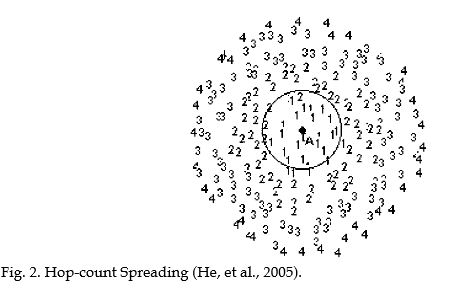
\includegraphics[width=200]{Proximity_estimation1.PNG} 
    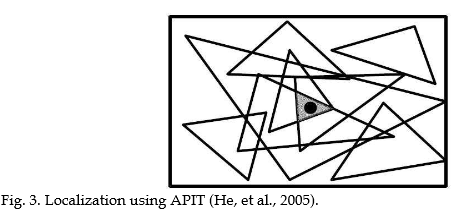
\includegraphics[width=200]{Proximity_estimation2.PNG}
    \caption{Proximity Estimation\cite{IndoorTrackingRSSI}}
    \label{fig:Proximity Estimation Diagram}
\end{figure} \\
    \item Triangulation Estimation - This is a method that uses a trigonometric approach into calculating the position of a target node. It requires two angles and the distance between them. This method uses trigonometry from the angle given and distance to target node. This can be seen in Figure \ref{fig:Triangulation Estimation Diagram}.
\begin{figure}[h!]
    \centering
    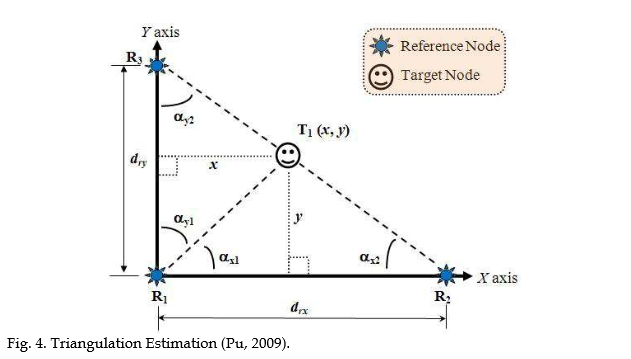
\includegraphics[width=225]{Triangulation_estimation.PNG} 
    \caption{Triangulation Estimation\cite{IndoorTrackingRSSI}}
    \label{fig:Triangulation Estimation Diagram}
\end{figure} \\
    \item Trilateration Estimation - This method uses the same technique as Triangulation, however, this method uses three reference nodes that are randomly allocated. These nodes emit a circle, which can be allocated as a range between the node and the target node. Knowing the position between each node, we can then work out the target node location from the distances given from each of the nodes. Pythagorean theorem can be used to calculate the coordinates of the target node. This can be seen in Figure \ref{fig:Trilateration_Estimation}. \\ 
\begin{figure}[h!]
    \centering
    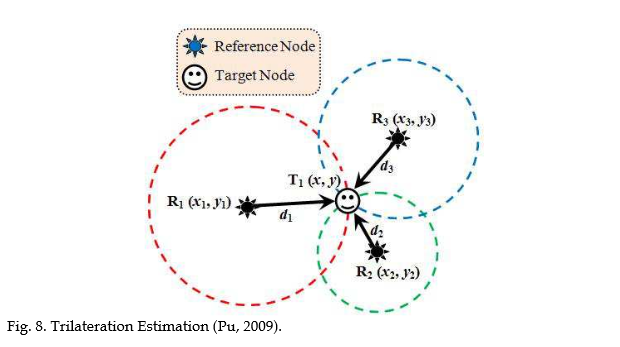
\includegraphics[width=225]{Trilateration_Estimation.PNG} 
    \caption{Trilateration Estimation\cite{IndoorTrackingRSSI}}
    \label{fig:Trilateration_Estimation}
\end{figure} \\
\end{enumerate}{}
The report then goes into discussing the RSSI to distance value and using the radio signal strength ranging equation to calculate the distance and using the received power and environmental power to work out the distance conversion to a higher accuracy. The environmental power was used to reduce the amount of error found within the conversion between the RSSI to distance. As depending on the environment that the device is placed in the signal strength received changes due to the radio signals having to go through walls and other objects. This would have an affect on the position tracking as the amount of error will be proportional to inaccuracy in the different methods used, as the calculated distance will be off by x amount.   The graph used to display the change in the environmental factor can be seen in Figure \ref{fig:RSSI vs Distance Diagram}. The report also discusses a formula that would be used to calibrate this factor. \\ \newline

\begin{figure}[h!]
    \centering
    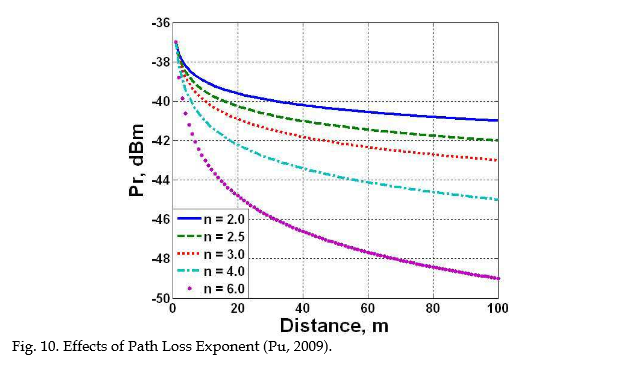
\includegraphics[width=250]{Indoor_locational_tracking_RSSI_Distance_graph.PNG} 
    \caption{RSSI vs Distance Diagram\cite{IndoorTrackingRSSI}}
    \label{fig:RSSI vs Distance Diagram}
\end{figure} \\

The final experimentation showed that RSSI could be used to track a mobile devices location, however, as the report states "With the existing technology, RSSI ranging is still not a perfect solution for fine-grained location tracking because of inaccurate and uncertain input data when it is used in on indoor environment."\cite{IndoorTrackingRSSI}. Nevertheless, even though their research shows that the method of using RSSI as an element for position tracking inside a building as being inaccurate, the method will still be useful within this project to provide further information on what data can be collected from mobile devices. It is one of the core variables that can be collected from packets being sent between two devices that indicates the device location. In this case, for this project, there will need to be further research or experimentation done to enhance the quality of the RSSI signal to distance conversion. Even though this is the case, the research conducted by Dongseo University provides three methods of position tracking that can be useful later in the project. Whilst the position tracking techniques are being developed research will need to be done about which technique would be best to use. An issue with this article that will also need to be considered is that the article position tracking techniques only consider the x and y axis. This means the z axis, the height, is not considered, therefore if there are multiple floors or uneven ground in a event the location accuracy could affected by this. As the distance will be altered by height.\\ \newline 

\section{Summary}
The literature goes into different key aspects for this project, that could be used to influence the development of the project. The information that was learnt will be taken into throughout the development of the product is: 
\begin{enumerate}
    \item When the MAC address is combined with other information, it will become personal data.
    \item Consent may be required to collect MAC addresses and additional data.
    \item Promiscuous mode\cite{Promiscuous_mode} can be used to collect MAC addresses and the signal strength of a intercepted packet.
    \item The hardware components attached to the microcontroller can affect the accuracy of the product.
    \item A network of data collectors can be used to record different routes that are taken in a set area or popular locations.
    \item Proximity, Triangulation and Trilateration can be used to work out the position of a target node. However, further research will need to be completed to work out difference in height.
\end{enumerate}


%-------------------------------------------------------------------------------------------------------
% Project Development
%-------------------------------------------------------------------------------------------------------
\chapter{Product Development}
The next stage of the project was to create the product that would approximate the amount of people in its surroundings through the mobile devices and producing a Data Processor that will take the data collected as an input to create useful statistics and visualisations. Within this chapter there are several core features of development, each of these stages will need to be designed and implemented. These components are: 
\begin{itemize}
    \item Database Architecture
    \item WiFi Counter
    \item Importing Data
    \item Visualisations
\end{itemize}
The features contribute to the full design of the product. Once the stages have been designed and built, different tests are required to ensure the product is working correctly and can function together to create the Data Collector and the Data Processor. The product is being developed to ensure that the set up can be used for future tasks outside of this project. Therefore, the code that is produced must follow a certain methodology and standards to ensure that the deliverables are flexible and adaptive to modification for future development as there are multiple areas where a product of this nature can be used for data gathering and analysis. This can be done by using the agile methodology method feature driven development (FDD) and backups to ensure that the work is secure.
\clearpage

%-------------------------------------------------------------------------------------------------------
% Ethics
%-------------------------------------------------------------------------------------------------------
\clearpage
\subsection{Ethics Clearance}
The first task to complete within the development of the project is to gain ethical clearance to conduct the project. This will allow for testing to be conducted within the rules set and to gather data during these tests to be used later on in the data processing stage of the project. However, a core problem that has determined what can be seen throughout the project is that the project has not been given ethical clearance. \\ \newline
The reasoning for this is due to the first ethical clearance form being rejected and having to be resubmitted under a new rule set. This would have not been a problem if the ethics committee made decisions within a week or two of submission, however, due to the time of year some of the core members of the committee were absent for a period of time. The ethics form was rejected in this scenario because the personal data that was being collected wasn't handled appropriately and people who were included within the testing grounds were not giving consent to collect the data from their mobile devices. \\ \newline
The two pieces of personal data that were being collected was the MAC address and time when the packet was read, to protect this the data collector would apply a MD5 hash against the MAC address to anonymise the data collected\cite{MD5}. In spite of that, the initial form did not count recording time as personal data. However, further consideration into the rejection showed that the time is personal data. As the dwelling time of a person in a certain area counts as a behaviour pattern towards that person and could identify them. The MD5 hash was also counted as not significant enough protection as if you know the persons MAC address that you are looking for you can apply a MD5 hash to it and match it with the dataset collected. Therefore, in the next submission of the ethics form the main change that was made was to gain consent from a participant to gather information about their mobile device. Then the data collected will be removed once the project has finished. Another modification to the report that had to be made was to clarify that all participants will be over 18 years old.\\ \newline
As the projects ethical clearance was not given a successful pass till the end of the project, the amount of tasks and tests that could of have been conducted were significantly reduced. \\ \newline 

\clearpage
%-------------------------------------------------------------------------------------------------------
% Database
%-------------------------------------------------------------------------------------------------------
\section{Database Architecture}
The database is the backbone to this project as it represents the structure that the product will take throughout the coding stages. The database architecture will determine how time expensive the final process will be. For this reason the database architecture design and implementation stages had been looked into first as the other components will be designed from the database architecture. Designing the database to be efficient is vital to ensure fast inputting and processing time. This will require looking towards different database management systems and optimisation techniques to support the efficiency of the final product. 
\subsection{Design}
The initial stages of the database architecture design requires an understanding of what variables are being stored within the database. The variables will then help to determine the database management system (DBMS) and then the architecture of the database through normalisation, restraints and CAP theorem\cite{CAPTheorm}. Therefore the variables that will decide the architecture of the database are:
\begin{itemize}
    \item MAC address\cite{MacAddress1} - the MAC address of the device being recorded. A one-way hash will be applied to the MAC address, to anonymise the personal data and reduce the chance of the MAC address being connected to the device holder. The Privacy Company states that the only data that can be collected from knowing a MAC address is the vendor information. This means that the information that counts as personal data is the dwelling time as it is recognised as behaviour patterns under GDPR (2018)\cite{GDPR}. 
    \item RSSI\cite{RSSI} - signal strength  for the connection between the tracker and the mobile device.
    \item Timestamp - time and date of when the reading was taken. 
    \item WiFi Counters MAC address -  This is the MAC address of each WiFi Counter and will be used as a unique identifier. 
\end{itemize}
Now the key variables have been stated the next task is to determine which DBMS will be used. There are a variety of DBMS to select from to store these variables, such as a document orientated or relational DBMS. The relational DBMS would be the best fit for this type of data as the values are always fixed variables and information. Hence there should be no redundant values through null or unwanted values. Therefore, document orientated DBMS is not an optimal choice as they allow for multiple records with different variables to ensure that the database can handle a mixture of values from each record, whereas the variables within this project do not have variety and are always fixed to a certain set of attributes.\\ \newline
This reduces the amount of DBMS down to one category of research which is SQL database and not NoSQL databases\cite{SQLvNoSQL}. These DBMS will be required to be used in either Arduino or Python. The DBMS that follow these requirements are:
\begin{itemize}
    \item MySQL \cite{MySQL} - The relational DBMS that contains a predetermined scheme for incoming data. Meaning that the data handed to the database must be fixed, to reduce redundant data.
    \item SQLite\cite{SQLite} - This is a simplified version of MySQL allowing for simple commands and processing. However, the main problem that resides with this language is that it struggles to handle multiple calls at once. Meaning if a lot of data is coming in the database may become locked.
    \item PostgreSQL\cite{PostgreSQL} - This language is an open-source version of MySQL with some differences. PostgreSQ is more supported of extensibility  and technical standards. Meaning the DBMS can be used on one device to a warehouse full of servers. 
\end{itemize}
The DBMS that would best support the project are MySQL or PostgreSQL as it can function with multiple commands at the same time, increasing the efficiency in which data is imported or processed. Whereas, SQLite cannot due to its simplified nature. PostgreSQL is a powerful version of MySQL, however, only by a tiny amount and they both have a lot of similarities\cite{PostSQLvsMySQL}. PostgreSQL would be useful for this project but could be seen as too heavy duty as the application will not be ran on multiple servers. Therefore, MySQL was chosen for the DBMS.\\ \newline
The next stage in designing the database architecture is to create a database architecture from the variables that were mentioned. This can be done through normalization\cite{Normalization} to reduce the amount of redundancy throughout the database. The normal form that all database want to be at is third normal form, the rules that must be followed are as stated:
\begin{enumerate}
    \item First Normal Form - it should have single atomic valued attributes.
    \item Second Normal Form - it should have functional dependencies. This is where attributes are dependent on a single attribute and will create a candidate key.
    \item Third Normal Form -  it should not have any transitive dependencies. There must be no attributes that rely on a non-primary attribute. 
\end{enumerate}{}
For this system to work each normal form stage relies on the previous stage to be implemented. The database architecture that was designed into normal form can be seen in Figure \ref{fig:ER_diagram}, which is an ER diagram that shows the relationships between tables in the database. This design is in third normal form because all attributes have a single atomic value. Secondly, each attribute is either a candidate key or functionally dependent on one. Finally all attributes are dependent on a primary attribute. \\ \newline 

\begin{figure}[h!]
    \centering
    \includegraphics[width=300]{er_diagram.PNG} 
    \caption{Entity Relationship (ER) diagram}
    \label{fig:ER_diagram}
\end{figure} 

There has been certain constraints applied throughout the database architecture to ensure consistency within the database and these are: applying 'Not Null' constraints where required. This will ensure that there are no null values throughout the database. As well, there are varchar limits included to ensure all strings do not go over a certain size. \\ \newline
\clearpage
\subsection{Implementation}
The database architecture implementation is the next stage of the project. This allows the project to proceed into the development of a data importer and analysis. The implementation of the databases architecture was done in parallel with the WiFi Counter to reduce the amount of time each feature would take. The database architecture was built using MySQL Workbench\cite{MySQLWorkbench}, which is an application that helps to configure MySQL servers and helps to create databases with ease. An example of this is shown in Figure \ref{fig:MySQL_Workbench}. After all the values were entered into the application, this would create a SQL script to make the table using the requirements set. This script was executed to make the table and at the same time was copied into a text file to be used in the python 'DBManager' object. \\ \newline
\begin{figure}[h!]
    \centering
    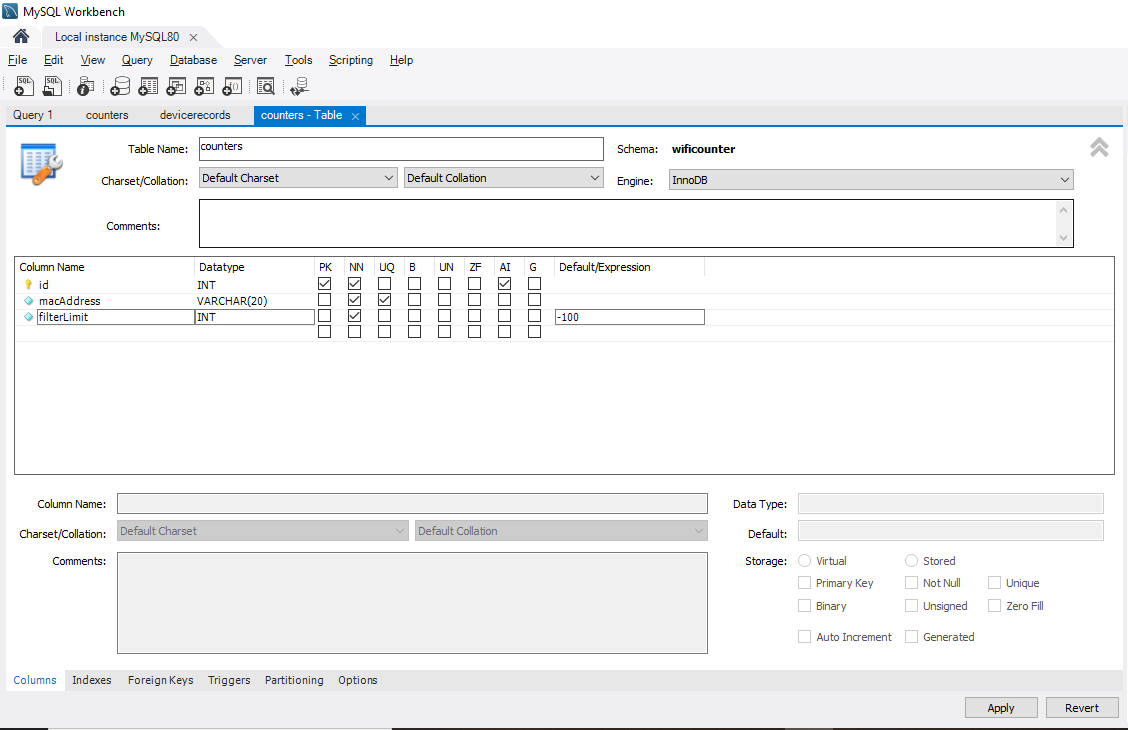
\includegraphics[width=200]{MySQL_workshop_1.PNG} 
    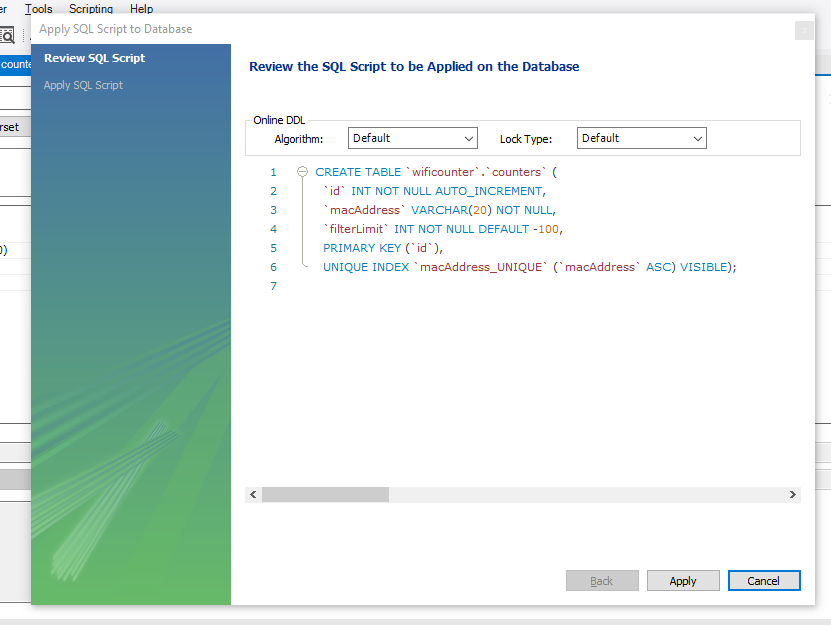
\includegraphics[width=160]{MySQL_workshop_2.PNG} 
    \caption{MySQL Workbench Table Creation\cite{MySQLWorkbench}}
    \label{fig:MySQL_Workbench}
\end{figure} \\
The 'DBManager' is an object that was written in Python for the purpose of communicating to the database. The library used to connect to the MySQL server was 'mysql.connector' and this allowed it to then execute queries to either collect or register new data to the database. The class diagram shown in Figure \ref{fig:class_diagram} shows the methods that were designed to manipulate the database as seen fit. The key methods in the object are 'db\_execute()', 'reset\_tables()' and 'is\_tables()' this is because they allowed for simple manipulation and checking whether the required tables were in the database. The execute command simply takes an input string and executes it to the database, you will have to state whether the output is being returned using the is\_output parameter, which is a Boolean. The 'is\_tables()' checks whether all tables needed for this application are within the database and if not reports an error, if an error occurs the  'create\_tables()' method can be used to create the tables required for the application to work. This is done through the SQL commands that were saved during the MySQL Workbench table creation phase. Finally, the 'reset\_tables()' sets the database record back to zero and resets the auto incremented id's to zero, this is done through using the 'TRUNCATE 'table name';' command and turning off the foreign keys to avoid errors. \\ \newline
\clearpage
\begin{figure}[h!]
    \centering
    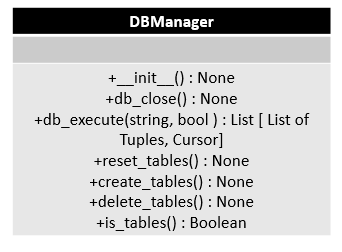
\includegraphics[width=200]{dbmanager_class_diagram.PNG} 
    \caption{DBManager Class Diagram}
    \label{fig:class_diagram}
\end{figure} \\
This completes the implementation of the database architecture. The 'DBManager' class allows for the object to be passed throughout any of the code developed and is used to communicate with the database. The methods also allows for easy manipulation of the database and enforces checks to ensure everything is set up correctly within the database. The object also reduces the amount of duplicated code within the project and ensures the application only needs to connect to the database once. As the database architecture is now developed and implemented into the product, the first deliverable has been achieved, which is an efficient database with a reliable method to communicate and manipulate the database as seen fit, the next stage is to focus on the WiFi Counters development, which will be collecting the data that will be going into the database that was designed.

\clearpage
%-------------------------------------------------------------------------------------------------------
% WiFi Counter
%-------------------------------------------------------------------------------------------------------
\section{WiFi Counter}
The WiFi Counter is the data collector that will collect the variables that will be stored in the database and this data will also be used to create visualisation and statistical models. The WiFi Counter is a major element to the network that will be built between the individual devices, as it is the only source from which the data is being collected. The method that will be used to collect the data involves making several small devices from the ESP8266 using the Arduino IDE\cite{ArdinoIDE} to produce a WiFi Counter that uses promiscuous mode to intercept packets being sent between devices. From this you can collect the variables that are needed for the dataset. The following chapter will go through the designing and implementation of the device.
\subsection{Design}
The key elements to the design of the WiFi Counter are to look into what microcontrollers would be best to use throughout the development of the project, how to gather the information required and then developing a way to store the data collected. Therefore, the first stage is to look into the different type of microcontrollers that can be used in this project. These are:
\begin{itemize}
    \item Arduino Uno \cite{AduinoUno} - this is a open source microcontroller, which has digital and analog input/output pins. This allows for multiple expansion boards and other circuits to be added to the board.
    \item Raspberry Pi\cite{RaspberryPi} -  this is a computer that can run Linux. This microcontroller will be able to run Python, which is a language that is very powerful for processing and analysing data\cite{Python}.
    \item ESP8266\cite{ESP8266} - is a low cost WiFi microcontroller that will be programmed using the Arduino IDE\cite{ArdinoIDE}. Therefore the microcontroller could be used to make the counter that will gather information about mobile devices within the vicinity.
\end{itemize}{}
All the microcontrollers have the ability to enter promiscuous mode, however, the ESP8266 is the best choice, as it already has a connection to the WiFi and is a cheaper microcontroller to the rest. This is useful as to make a network of devices that can cover a large area you will need multiple WiFi Counters set up in the location where the mobile devices are being tracked. Even though the Arduino Uno was used in the 'WiFi Tracking Using Arduino WiFi Shield'\cite{ProtrackingArduino}, to make the network functional a  WiFi Board will need to be included. As well, the report showed that even though the project worked, the Arduino Uno set up only performed well in an area which has few access points. Experimenting with using the ESP8266 as a WiFi tracker could overcome this problem or have a better advantage over the Arduino board as the ESP8266 are designed to connect to the WiFi. \\ \newline
After the decision was made to use the ESP8266, two tasks were left to complete. Further research into how promiscuous mode worked and to find a method to store the data collected. Promiscuous mode works by allowing the network device, the ESP8266, to intercept and read each network packet that arrives in its entirety\cite{Promiscuous_mode}. Knowing this, we must ensure the only data that is collected when recording the intercepted packet is the MAC address of the sender or receiver and the RSSI\cite{RSSI} to ensure that no data that could be connected to the device holder is being collected. The other key variables that need to be collected can be found through ESP8266 hardware instead of reading any further information into the packet that was intercepted. Knowing this, the final part to design for the WiFi Counter is how to store the data, there are a couple of options that would provide a solution to this. These are:
\begin{itemize}
    \item SQL Database - a SQL database familiar to the Database Architecture chapter. This can be used to store the data gathered in a database in the same format on the ESP8266.
    \item SD Card Storage - this is a memory card that is used within portable devices. This form of storage will make the data collected portable to other hardware devices.
    \item SPIFFinFile\cite{SPIFF} - this is a flash memory file system. It is a light-weight file system for microcontrollers with the Serial Peripheral Interface (SPI) flash chip and can store 1-4MB of memory. 
\end{itemize}
The most efficient version of storage on the WiFi Counter is to use a SD card because the card can be transported between hardware devices. This means that the locations where there are no WiFi connections nearby, you can then take the card from the WiFi Counter and save the data recorded on the device that the Data Processor application is on. The alternative methods are both strong methods of storing data, however, both are stored onto flash memory so that the data cannot be sent to the Data Processor without connection to the WiFi. \\ \newline
The WiFi Counter will also need to be efficient while completing tasks in the code. This is because the more complicated extra steps can be equivalent to time that would intercept possible packets through promiscuous mode. If these packets are missed the dataset that is produced at the end of the run time could be less valuable, as the packet missed could have indicated a mobile device that is still nearby and has not left the range of the WiFi Counter. This loss would therefore reduce the richness of the dataset that is produced. Therefore, when producing the code this fact must be considered and the functionality of the code must be kept to standards. \\ \newline
The final design for the WiFi Counter consists of using a ESP8266 board to collect the required information and a SD/Micro SD card to store the data. This device will then be used in different environments to track mobile devices and collect a dataset of what devices were seen through the run time. The device consists of multiple low price components to ensure multiple WiFi Counters can be manufactured and used throughout a network to produce a set of data in different sized areas. The device to be portable will need a battery bank and a case to ensure it can be powered and stored safely in different environments.  \\ \newline

\subsection{Implementation}
The implementation of the WiFi Counter took several stages to complete the deliverable as it is one of the more complex items in this project. The reasoning behind this is that the device is the collector of all the data throughout the project. As well, if the data gathered is incorrect the richness of dataset will be reduced. The stages of implementation for the WiFi Counter were:
\begin{itemize}
    \item Enabling promiscuous mode and gathering key variables
    \item Reading and sending data to the SD card
    \item Filtering the MAC addresses
\end{itemize}
These implementation stages will be separated into sections to fully understand how the different sections were implemented. However, there were two key issues with the development of the device which originated from the same error. This was a 'Soft WDT Reset'\cite{SoftWDTReset} which has two different causes, which are an exception error or watch dog timeout error. In the process of coding the WiFi Counter both of these versions of error were found and one still remains. These errors were found when doing:
\begin{itemize}
    \item Exception error - The error occurs when code is performing illegal operations. The illegal operation that was being conducted to cause this error was calling a string memory location that was null. This is due to the heap fragmentation created by the string variable. This is because as the string items are replaced the items sizes are not reorganized to be able to stack string on top of each other but are simply placed in the old gap, this therefore can leave tiny spaces of memory that cannot be reallocated due to then memory size\cite{String}. This is a major issue on Arduino and ESP8266 due to small amount of RAM on the devices that is allocated to constant variables. This was fixed by changing all string variables to char arrays, which allocate memory space more efficiently. However, the code developed had to be restructured to be able to handle char arrays instead.
    \item Watchdog error - This error was caused by the code becoming stuck into a loop or had stopped for an x period of time. This problem was not fixed due to the location of where the error appeared, as it was where data was uploaded to the text file on the SD card. This meant that in some scenarios sending the data to the SD card would take too long and cause the Watchdog Timeout. A reason for this could be that multiple packets are intercepted within the same time frame, however, this caused a queue to build up which locked up the SD card to being open for too long. This would then cause a timeout error.   
\end{itemize}
Furthermore the change in code structure meant that implementing the code for the WiFi Counter took longer than originally planned. This was because to find and fix the error was time expensive. Therefore, the following sections discuss the core structure of the code that was implemented from the design stage after the modifications were made to help fix the functions. 
\subsection{Promiscuous Mode And Key Variables}
The first stage to collecting the different variables using the WiFi Counter is to enable promiscuous mode. This mode will monitor its surroundings for packets being sent between two different devices. This is done through using the command 'wifi\_set\_promiscuous\_rx\_cb()'\cite{activate_promiscous_mode} and 'wifi\_promiscuous\_enable()'\cite{activate_promiscous_mode}, these functions will set whether promiscuous mode is turned on or not and what function to call when a packet is intercepted. This callback function will collect the required information from the packet and then record the data to the SD card. \\ \newline
The structure for creating the callback function was inspired by  Łukasz Podkalicki in his article about creating a 'ESP8266 - WiFi Sniffer'\cite{promiscuous_mode}. The code within the article was used as reference to collect the receiver or sender MAC address and RSSI from the intercepted packet. The change between string to char array meant that a more simplistic method of writing the code was converted to more complex. This is due to the MAC address value needing to be converted from 'uint8\_t' to a hexadecimal value in char array form. This meant the function 'decToHex()' was made. This function works by taking the decimal value given and using the formula to convert an integer to hexadecimal into a char array representation. This can be seen in Figure \ref{fig:decToHex}. As the function to convert decimal to hexadecimal char array had been made, the next step was to combine the outputted values to represent a MAC address. This was done by creating a for loop that would append the hexadecimal char array to the MAC address char array with the ':' characters and changing the last value from ':' to '\textbackslash o' to indicate the end of the string. The final part of the callback function is checking that the MAC address is not null values, which look like 'FF:FF:FF:FF:FF:FF'. After this the valid MAC addresses are passed to 'recordData()' function with the RSSI value found in the packet. This can all be seen in Figure \ref{fig:callbackFun}.\\ \newline
\begin{figure}[h!]
    \centering
    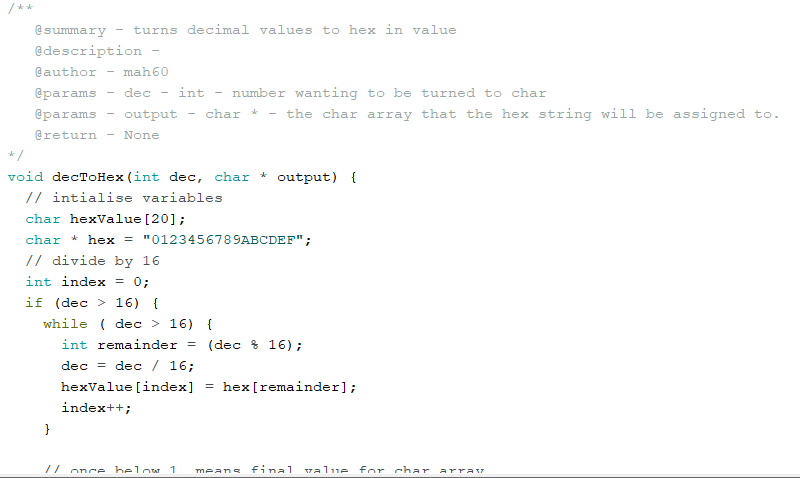
\includegraphics[width=200]{hexToDec_1.PNG} 
    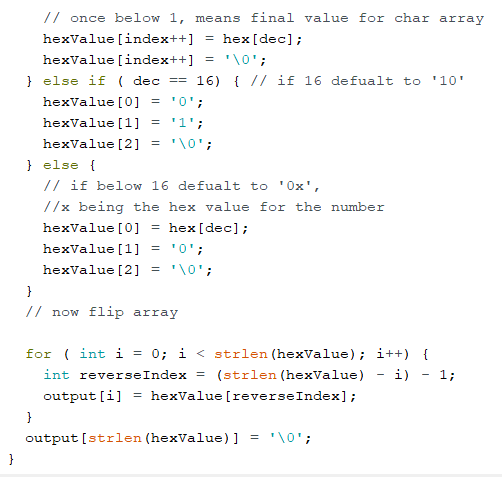
\includegraphics[width=200]{hexToDec_2.PNG}
    \caption{decToHex() Code}
    \label{fig:decToHex}
\end{figure} \\

\begin{figure}[h!]
    \centering
    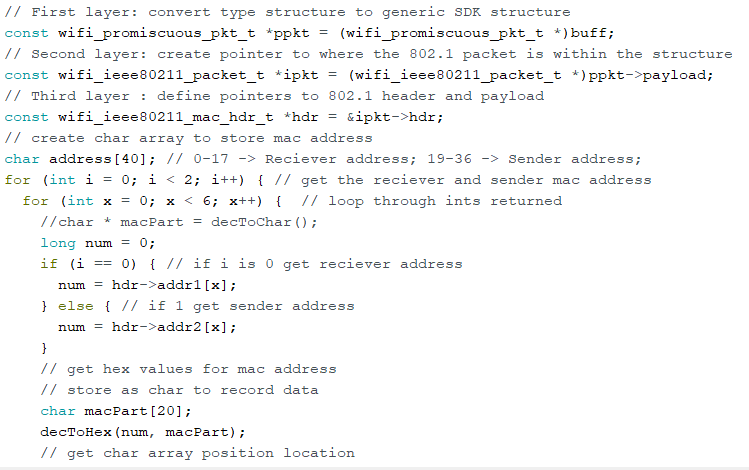
\includegraphics[width=200]{callback_1.PNG} 
    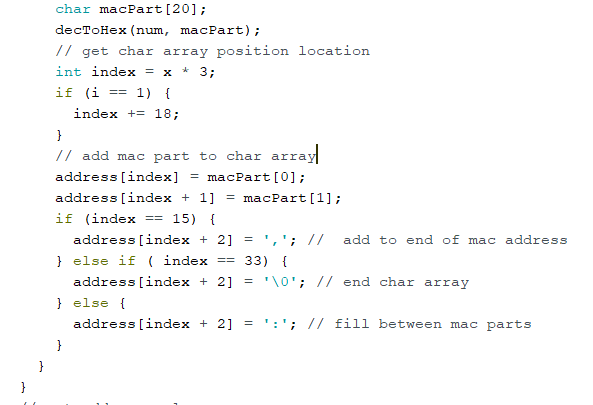
\includegraphics[width=200]{callback_2.PNG}
    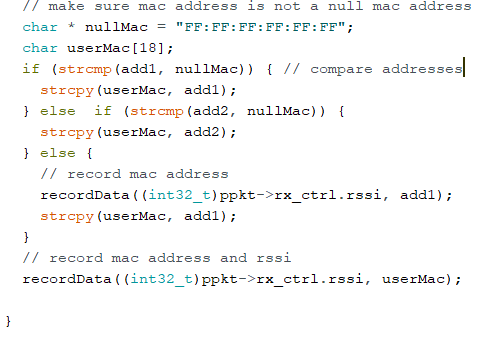
\includegraphics[width=200]{callback_4.PNG}
    \caption{Callback Function Code}
    \label{fig:callbackFun}
\end{figure} \\

The next step is to ensure that all the required values can be collected. The variables that have been gained through the callback function are the MAC address and RSSI value, this means that the remaining variables are the recording time stamp and the WiFi Counters MAC address. These are found in the setup function at the start of the run time, this was done by using the package 'NTPClient'\cite{NTPClient} to get the start timestamp using the function made by kaefert on the Github NTPClient issue blog\cite{getCurrentTime}. This function was then modified to handle char arrays instead of string, this was done through using the 'itoa'\cite{itoa} to convert the integer value to char array. The 'getTimeStamp()' returns a char array of the start timestamp. The function 'millis()'\cite{millis} was used in the 'getRunTime()', where the function would use 'millis()'\cite{millis} minus the start millis time to get the amount of seconds that the device has been running for, but excluding the start up time. This will then be used at a later date to be added to the start timestamp to get the timestamp of a packet that was intercepted. This was done as the ESP8266 has no internal clock without an attachment, which means that the timestamp cannot be set on the ESP8266 and the current time can not be gathered without a connection to the WiFi, which is always turned off when promiscuous mode is active. These functions can be seen in Figure \ref{fig:getTime}.\\ \newline
\clearpage
\begin{figure}[h!]
    \centering
    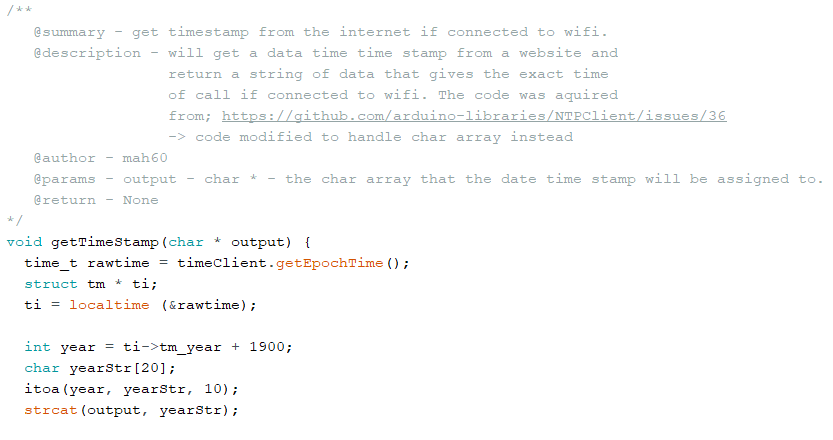
\includegraphics[width=350]{getTime_1.PNG} 
    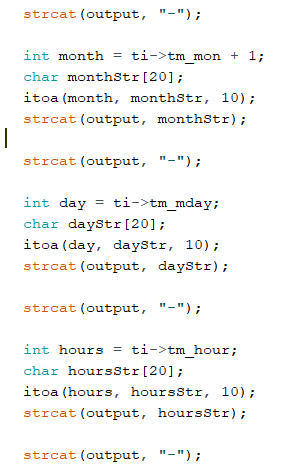
\includegraphics[width=100]{getTime_2.PNG}
    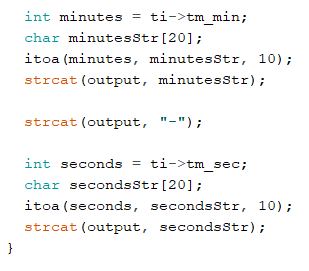
\includegraphics[width=100]{getTime_3.PNG}
    \caption{getTimeStamp() Code}
    \label{fig:getTime}
\end{figure} \\
The next step is to get the WiFi Counters MAC address, this is done by simply passing the function 'WiFi.macAddress()'\cite{wifMACaddress} and using the function 'decToHex()' that was used before to convert the bytes returned to a hexadecimal char array value and then appended to a char array for the WiFi Counters MAC address. As shown in Figure \ref{fig:decToHex}. The final stage process was to apply a MD5 hash to the found MAC addresses to anonymise and protect the personal data that was gathered. This was done by using the MD5 algorithm\cite{MD5} that is usually applied to passwords to ensure that they cannot be converted and only compared. This was done through the the MD5Builder\cite{MD5Builder} packet found in the ESP8266 library. This can be seen in Figure \ref{fig:recordData_MD5hash}. Alternative methods were considered, such as AES encryption using the Crypto\cite{AESEncryption} library. However, this was believed to be an unreliable method to protect the data collected as if the data was encrypted, the data could then be decrypted using the same method. Whereas, MD5 one-way hash meant that the MAC address could only be hashed and not converted back, this would then protect the data more than encryption as the MAC address could only be compared. \\ \newline
\begin{figure}[h!]
    \centering
    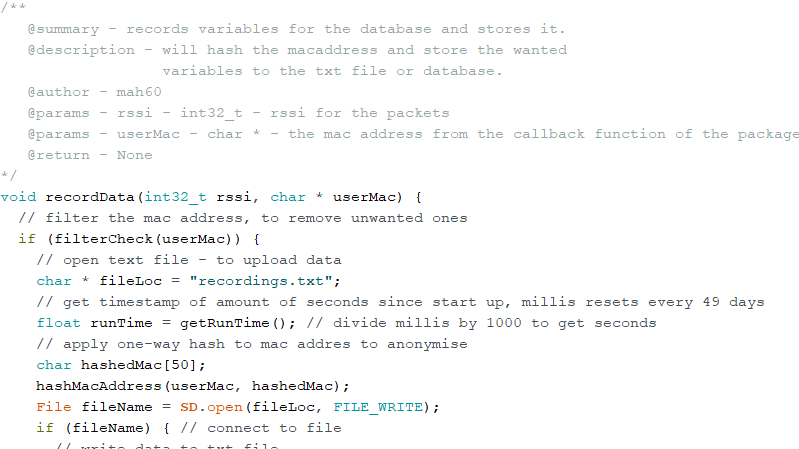
\includegraphics[width=400]{recorddata_1.PNG} 
    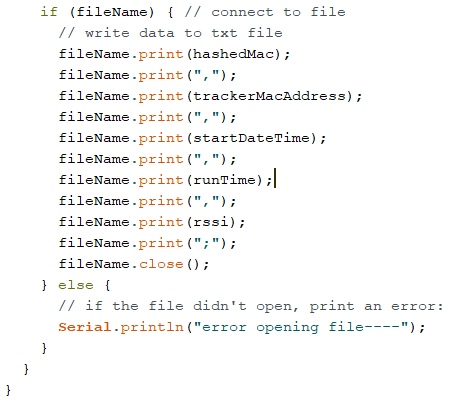
\includegraphics[width=200]{recorddata_2.PNG}
    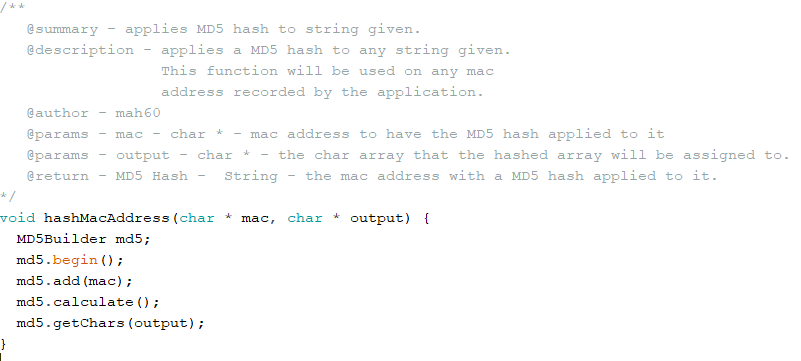
\includegraphics[width=400]{MD5_hash.PNG}
    \caption{recordData() & hashMacAddress() Code}
    \label{fig:recordData_MD5hash}
\end{figure} \\
\clearpage
\subsection{Micro SD Card}
As the data has been acquired, the next part to building the WiFi Counter was to store the data gathered. This part delayed the project due to the micro SD card modules taking two weeks to arrive. After they arrived the order in which the pins had to be connected needed to be worked out. This was determined, however, the pin that caused the main problem was the voltage pin, which is seen to be VCC on the micro SD card module to VV on the ESP8266 not VIN. The layout for the pins can be seen in Table \ref{tab:pin_layout}.  \\ \newline
\begin{table}[h!]
    \centering
    \begin{tabular}{c c}
    \hline
     ESP8266 Pin & Mico SD Card Module Pin\\
     \hline
     VV & VCC \\
     G & GND \\
     D6 & MISO \\
     D7 & MISI \\
     D5 & SCK \\
     D8 & CS \\
     \hline
    \end{tabular}
     \caption{Pin Layout}
     \label{tab:pin_layout}
\end{table} \\ \newline
The pin layout can also be seen in the circuit diagram in Figure \ref{fig:circuitDiagram}. As the micro SD card module is now connected to the ESP8266 the next task was to upload data to a text file on the SD card. This was done using the library 'SD'\cite{SD} and 'SPI'\cite{SPI} to first connect to the SD card and then upload data using the 'SD.open()' and 'file.write()' function. This code can be seen in Figure \ref{fig:recordData_MD5hash}. \\ \newline
\begin{figure}[h!]
    \centering
    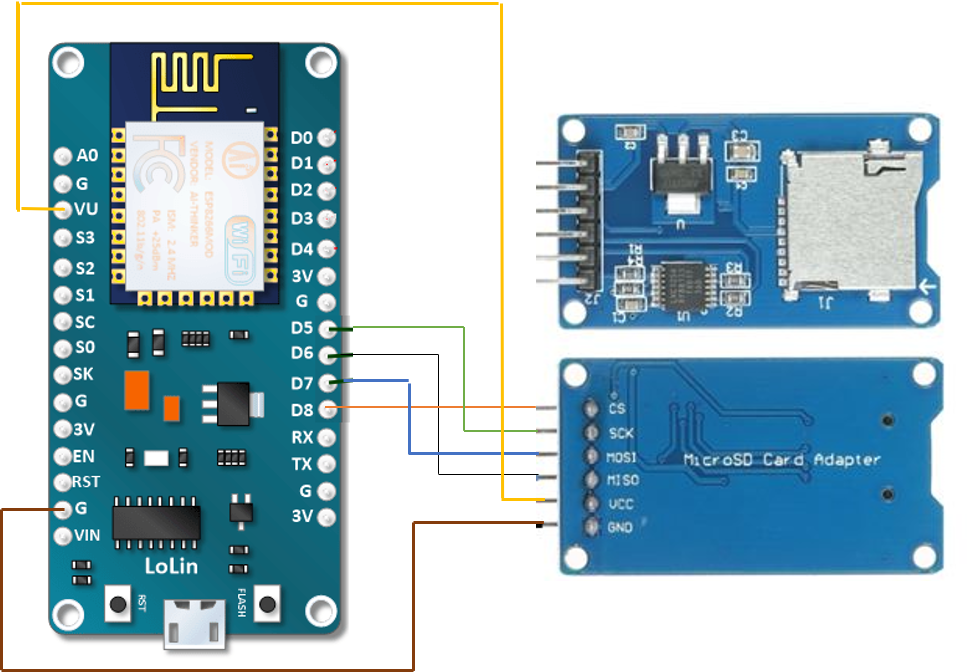
\includegraphics[width=300]{circuit_diagram.png} 
    \caption{Circuit Diagram}
    \label{fig:circuitDiagram}
\end{figure} \\
The code written in Figure \ref{fig:recordData_MD5hash} is where the watchdog timeout error is occurring. In spite of this, the WiFi Counter can now store a large amount of data using the micro SD card module and the format in which each recording is saved is in : "hashedMacAddress, WiFiCounterMacAddress, startDateTime, runTime, RSSI;". The recorded data will then be saved to the SD card and will be imported into the database by splitting the data up by the characters ',' and ';'.
\subsection{Filtering MAC addresses}
In consequence to the issue with the ethical clearance, a procedure that was issued to allow for ethical clearance is to filter the MAC address so that only participants will be read by the WiFi Counter. This was done by having a CSV file of MAC addresses on the SD card. The method 'getFilters()' was then called. To assign the MAC addresses to the 'filteredMacAddress' variable that can hold a total of fifty MAC addresses to filter. That variable is then supported by the two variables 'filterCount' to display how many filters are in 'filteredMacAddress' and 'commaLoc' will be the index values of where the commas are that split the MAC addresses up in the array.  The function 'getFilters()' works by reading the CSV file character by character. Then replacing each newline with a comma to split the char array up by MAC address. At the end of the 'filteredMacAddress' a pointer to the end of the string is added to ignore any null values in the array. This is a long way to make an array of char arrays using the comma values as a pointer to where each MAC addresses starts and ends. This was done due to the string problem that was discussed and can be seen in Figure \ref{fig:wifigetFilters}. \\ \newline
\begin{figure}[h!]
    \centering
    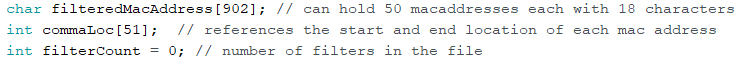
\includegraphics[width=300]{getFilters_3.PNG} 
    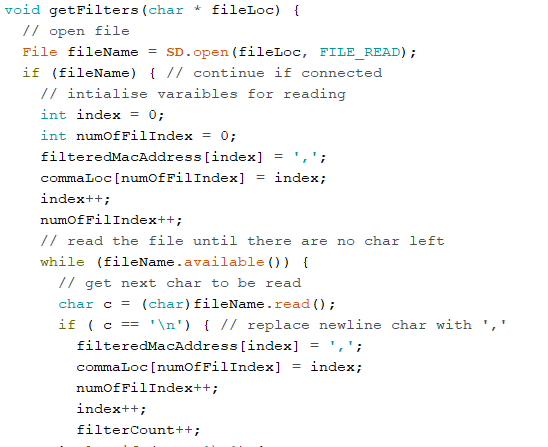
\includegraphics[width=250]{getFilters_1.PNG}
    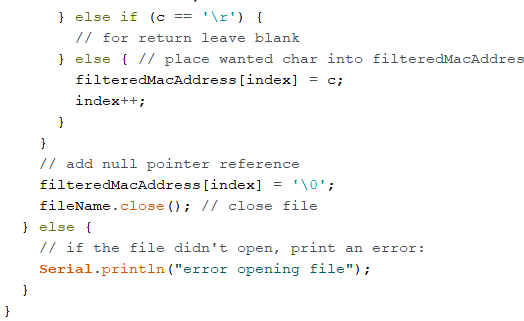
\includegraphics[width=250]{getFilters_2.PNG} 
    \caption{getFilters() Code}
    \label{fig:wifigetFilters}
\end{figure} \\
The final part to the filter was to create a function that would filter out any irrelevant MAC addresses. This was done in the function 'filterCheck()', which used 'filterCount' for the amount of times to loop through and used the function 'getCharInRange()' this function put only the values between two indexes into the output char array. Then the 'filterCheck' function would return a boolean to indicate whether the MAC address should be recorded. These functions can be seen in Figure \ref{fig:charRange_filterCheck} and were implemented into the 'recordData()' function as seen in Figure \ref{fig:recordData_MD5hash}. \\ \newline
\begin{figure}[h!]
    \centering
    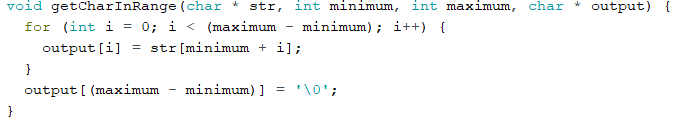
\includegraphics[width=300]{charRange.PNG} 
    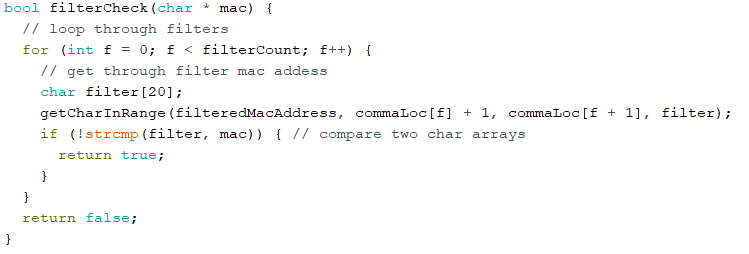
\includegraphics[width=300]{filterCheck.PNG}
    \caption{getCharInRange() & filterCheck() Code}
    \label{fig:charRange_filterCheck}
\end{figure} \\
This concludes the development of the WiFi Counter that will be used throughout the project to collect the data. The final build will be using a ESP8266 microcontroller and micro SD card module as hardware. These will record the data on the SD card in the format given, this can then be transported to any other hardware device and at a later stage have the device transmit the text over WiFi to create a dynamic network of devices to automatically upload data to the MySQL server, which can then produce reports from the data provided.\\ \newline

\clearpage


%-------------------------------------------------------------------------------------------------------
% Importing Data
%-------------------------------------------------------------------------------------------------------
\section{Importing Data}
The two primary elements of the product had been developed. They provided a method to store and manipulate the data gathered and we are able to create a dataset that will allow for us to research into what data can be gathered from mobile devices. However, to start looking into what data can be gathered from the dataset, the product needs a method to import the data collected from the WiFi counter to the MySQL database. This chapter will discuss the designing and implementing step for this. 
\subsection{Design}
The designing stage for importing data to the database will consist of looking at the format that the data is gathered in by the WiFi counter and then take the data and format it to go into the database. As explained in the WiFi Counters development the  string of data consists of this format : "hashedMacAddress, WiFiCounterMacAddress, startDateTime, runTime, RSSI;". This format is the same for each record. Therefore, when importing the text file into Python we can split the string built by the deliminator ';' for each record to make a list of strings. Then split each item in the list by the ',' deliminator to get the individual parts of the string that need to be recorded. The next step is to format the data gathered into a suitable format that will efficiently insert the data into the database with accurate and fast transactions. \\ \newline
The next stage required is to research into methods of inserting data. An article that was useful for research into this problem was a article by Eugene Philipov on 'insert vs insert many' queries\cite{insertRecords}. This article produced a graph of results that demonstrated that insert many were quicker than normal inserts into a database. However, doing a set size insert is better than a massive insert many. The research was conducted on one million records and these methods were done to a MySQL database, this can be seen in the diagram seen in Figure \ref{fig:charRange_filterCheck}. The bulk copy program (BCP) utility\cite{BCP} was shown to be the efficient method of importing data. This is because this system is designed to insert a large amount of data into the database. Therefore, this method is also applicable to insert records at a fast and efficient pace. This means BCP or insert many can be used to import the data to the database. \\ \newline
\begin{figure}[h!]
    \centering
    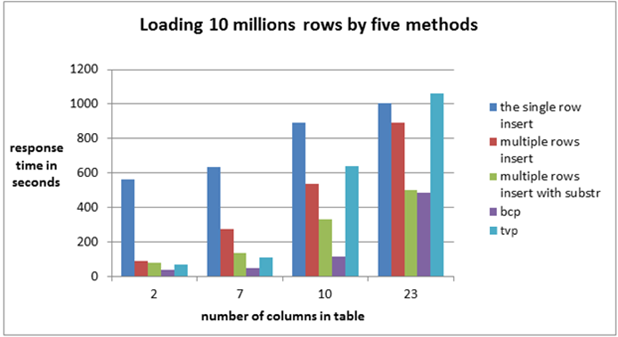
\includegraphics[width=300]{loadingDataGraph.PNG}
    \caption{Loading data using different methods\cite{insertRecords}}
    \label{fig:charRange_filterCheck}
\end{figure} \\
The next formatting issue is to get the recording time, as we have the start timestamp and current run time in seconds. These combined make the recording timestamp, however due to the problem that occurred from the 'soft WDT reset'\cite{SoftWDTReset} in WiFi Counter the run time is reset. To solve this there will need to be a total run time, which will add the previous value to the current total to stop the run time going back to zero. This method will cause a slight inaccuracy of when the device was recorded, however, this will stay insignificant until the device has been running for a week or two. This is because of how the WiFi Counter is set up, the start up time is taken away from the run time to make the value accurate to the 'getTimeStamp()' function on the WiFi Counter.\\ \newline
The final procedure is to look into a method that will filter out recordings outside the WiFi Counters set range. This could be done by using a mobile device in the time frame of the counters session, which stays stationary and calculating the average RSSI of that device in the time set for filtering. When the average is found applying a +x amount of error to reduce the amount of lost data that is still useful to the research. The error is added because the nature of the WiFi signal strength produced can vary by a certain amount, the noise of the surrounding environment. \\ \newline
The design is simplistic as the inputting of data to the database needs to format the incoming data into insert many statements or a BCP utility to allow for fast and efficient transactions between the database and data importer object. The other variable that must be considered in the implementation is to only execute a transaction that is lower than the max allowed packet size, which is 4MB, in bytes. This can be found through using the query 'SHOW VARIABLES LIKE 'max\_allowed\_packet';'. As possibilities have been looked into on how to insert the dataset gathered from the WiFi Counter to the database, the next step is to implement the methods discussed into the code in Python. \\ \newline
\subsection{Implementation}
The code that was implemented, had to complete three key stages. This was to get the data from the text file and split the data by record, then format the data into insert many queries and afterwards create a filter from the data given to the config file. There was an attempt to implement BCP utility into the code for importing data, however, the bcpy object\cite{bcpy} could not connect to the database to import the data. Therefore, insert many queries was used instead. \\ \newline
The record handler is the object that will use the method 'import\_txt\_to\_db()' to import the data from the given text file location. The method starts by using the function 'read\_txt\_file()' to read the data into a list of strings split by the deliminator ';'. The code for this can be seen in Figure \ref{fig:read_Text_file}. Each record in the text file was then split by the ',' deliminator. After this, formatting begins to add to the insert many query strings. \\ \newline
\begin{figure}[h!]
    \centering
    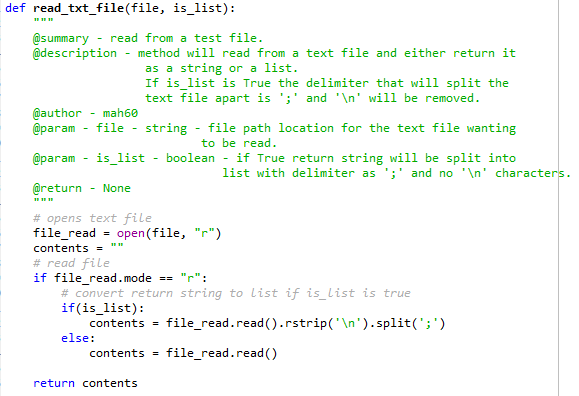
\includegraphics[width=250]{readTxtFile.PNG}
    \caption{read\_txt\_file() Code}
    \label{fig:read_Text_file}
\end{figure} \\
The formatting consists of making checks and ensuring any data sent to the database is correct and to ensure that no errors are caused when executing the queries or any redundant data added to the database. The first stage is to check that if the start timestamp is null, in this case the value will be set to the year '1970', then if the value is null the value set in 'config.start\_date\_time' will be used. The next stage is to go through each part of the record and add it to the insert many queries. This begins with the device hashed MAC address, this insert query needs to ensure that there are no duplicates, this is done by having a list of unique MAC addresses and checking the database for what MAC addresses are already in the device table. This is done using if statements and also gathers an ID number for the different MAC address and if a new MAC address is found, it adds the ID and MAC address to the list. The MAC address is also added to the device tables query. This can be seen in Figure \ref{fig:read_txt_constants}.\\ \newline
\begin{figure}[h!]
    \centering
    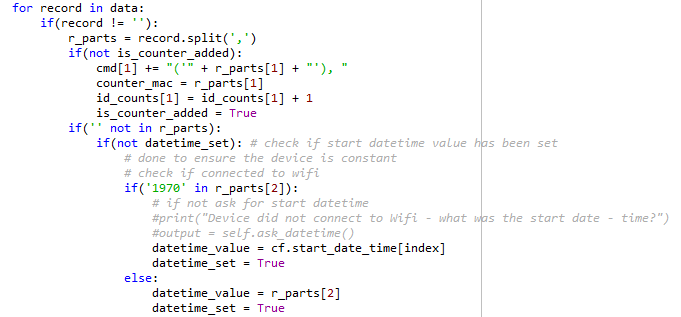
\includegraphics[width=250]{constant_set_up.PNG}
    \caption{Read Text File Constants Set Up Code}
    \label{fig:read_txt_constants}
\end{figure}{} \\
The next step is to create the recording timestamp, which uses a total run time to counter the watchdog resets in the WiFi Counter. This method can be also used when the error is fixed, as millis resets after forty-seven days due to the value going over the max byte size for an integer on the ESP8266. To make the recoding timestamp the total runtime must be added to the start timestamp. This can be seen in figure \ref{fig:read_txt_rec_timestamp}. This data along with the records RSSI and the counterId is added to the recordings table query. The next stage was simply to add the deviceId and recordId to the devicerecords table query.\\ \newline
\begin{figure}[h!]
    \centering
    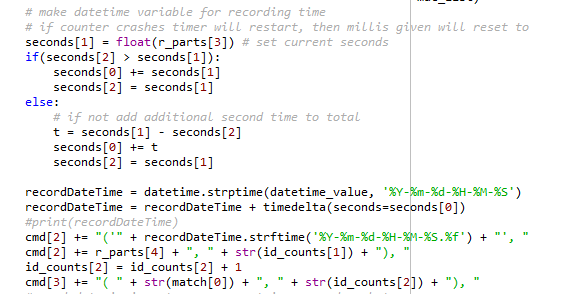
\includegraphics[width=250]{read_text_file_recording_timestamp.PNG}
    \caption{Read Text File Recording Timestamp Code}
    \label{fig:read_txt_rec_timestamp}
\end{figure}{} \\ \clearpage
Once the formatting was complete, it was time to execute the insert many command. This would be done once the string got above a certain size of bytes, which was calculated from an experiment with the time it took depending on the byte cap. This was done as the article by Eugene Philipov\cite{insertRecords}, discovers the size of the records sent in the insert many command alters the time taken to import the data to the database. He finds out that sending all the data at once is not the most efficient way to send the data as sending it in batches will reduce the load put on DBMS and reduce the time taken to complete the query. Through testing the best byte cap size changed due to the record size, the most optimised byte cap is proportional to the amount of records. For example, with 48K records a cap size of 250K is best, whereas, with 180K records a cap size of 500K is better. This can be seen in Table \ref{tab:Byte cap optimisation}. The method to insert the data would be done using 'send\_records()' method which would take the list of commands and use the DBManager given to this RecordHandler object to execute the statements. This can be seen in Figure \ref{fig:byte_cap_read}.\\  \newline
\begin{table}[h!]
    \centering
    \begin{tabular}{|c|c|c|c|c|c|c|c|c|c|}
    \hline
             & \multicolumn{9}{|c|}{Results (Seconds)} \\ 
        \hline
         & \multicolumn{3}{|c|}{48401 Records} & \multicolumn{3}{|c|}{179900 Records} & \multicolumn{3}{|c|}{446377 Records} \\
    \hline
        Byte Cap & Test 1 & Test 2 & Test 3 &  Test 1 & Test 2 & Test 3 & \vline Test 1 & Test 2 & Test 3 \\
    \hline
        4000K &  88 & 92 & 102 & 615 & 618 & 615 & 1851 & 1845 & 1852 \\
        2000K &  91 & 89 & 88 & 390 & 388 & 393 & 1183 & 1174 & 1176 \\
        1000K & 69 & 56 & 49 & 274 & 263 & 265 & 752 & 761 & 747\\
        750K & 46 & 46 & 67 & 249 & 245 & 248 & 727 & 733 & 727 \\
        500K &  44 & 45 & 44 & 242 & 240 & 241 & 793 & 801 & 752 \\
        250K & 65 & 45 & 46 & 229 & 233 & 235 & 822 & 782 & 776\\
        100K & 51 & 65 & 79 & 282 & 241 & 247 & 948 & 933 & 837\\
        10K & 137 & 133 & 149 & 485 & 517 & 477 & 1046 & 1214 & 1320 \\
        \hline
    \end{tabular}
    \caption{Byte cap optimisation experiment}
    \label{tab:Byte cap optimisation}
\end{table} 
\begin{figure}[h!]
    \centering
    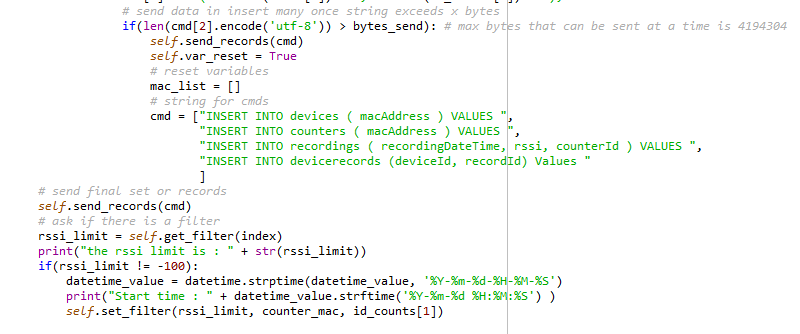
\includegraphics[width=250]{read_text_file_byte_cap.PNG}
    \caption{Read Text File Byte Cap Code}
    \label{fig:byte_cap_read}
\end{figure}{} \\
The final stage on importing the data was to filter devices out of the range given. The config file would take input for each record list added, this would be either '["None"]' or ["device MAC address used", "start timestamp", "end timestamp"] as seen in Figure \ref{fig:import_data_config}. The method to filter the data will be done after the data is inserted to the database. Then the code will check if the filters variables are equal to "None". The default value is then applied and if no average RSSI can be determined, the default value is -100. Then the MAC device given is checked by applying the MD5 hash to the value given through the hashlib library\cite{hashlib} and then compared against the database to ensure the MAC address exists. The next stage is to create a query that checks between the start and end timestamp and gets the average RSSI using 'ROUND(AVG(recordings.rssi))' select query. This can be seen in Figure \ref{fig:get_filter}. The RSSI value is then returned and noise error rate is added to the final RSSI filter limit. \\ \newline
\clearpage
\begin{figure}[h!]
    \centering
    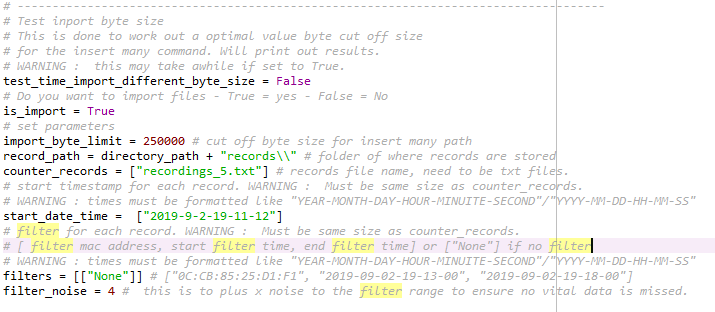
\includegraphics[width=250]{config_import.PNG}
    \caption{Import Data Config Code}
    \label{fig:import_data_config}
\end{figure} \\
\begin{figure}[h!]
    \centering
    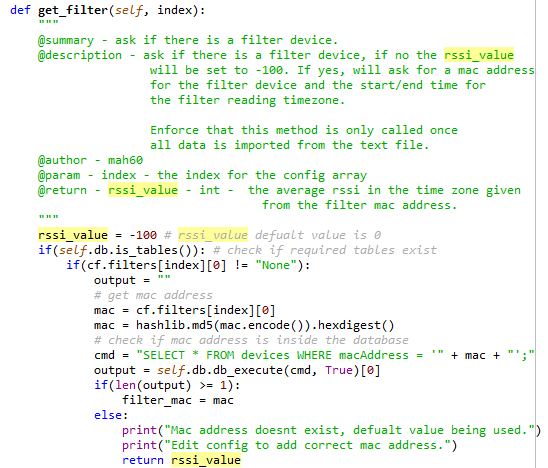
\includegraphics[width=225]{get_filters.PNG}
    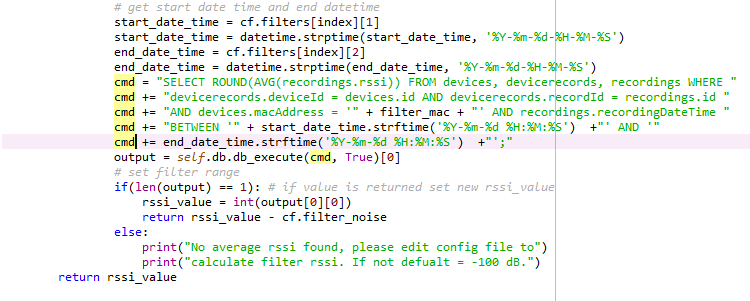
\includegraphics[width=225]{get_filters_2.PNG}
    \caption{get\_filter() Code}
    \label{fig:get_filter}
\end{figure} \\
The final task is to set the RSSI limit and ensure all records in the database do not go beyond this limit. This will be done with the 'set\_filter()' method if the RSSI limit is not set to -100. The functions starts by executing a query that will find all RSSI values that are greater than the RSSI limit and getting the 'recordings.id' and 'devicerecords.id'. The foreign key rules are deactivated to allow for records to be deleted from the database. Then a drop statement is executed for each ID found to be over the RSSI limit. Once this task is completed the RSSI limit is altered for that WiFi Counter and the foreign key rules are activated again. This can be seen in Figure \ref{fig:set_filter}.\\ \newline
\begin{figure}[h!]
    \centering
    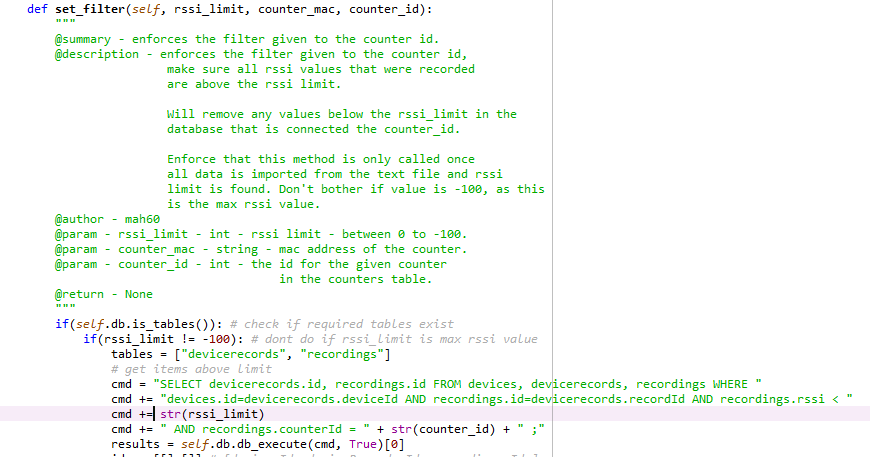
\includegraphics[width=225]{set_filters.PNG}
    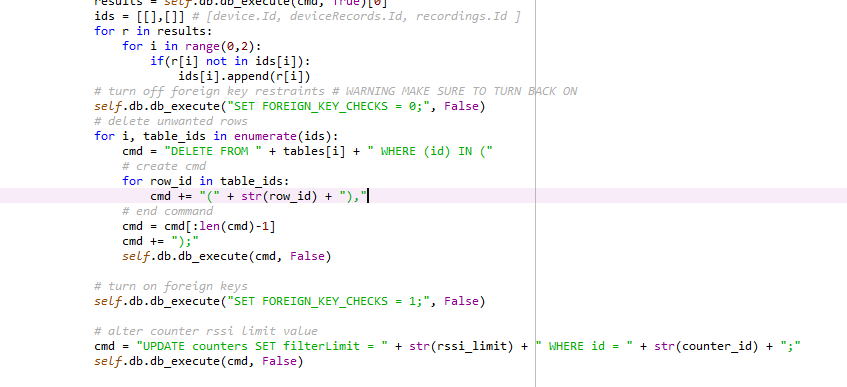
\includegraphics[width=225]{set_filters_2.PNG}
    \caption{set\_filter() Code}
    \label{fig:set_filter}
\end{figure} \\
With this the final tasks for the data importer are implemented. The  RecordHandler can now import data to the database through the 'import\_txt\_to\_db()' function, which formats the text file to be ready to be inserted into the database. A filter is then applied to the database if stated in the 'config.filters' variable. However, the import time can take a few minutes. This is due to the formatting to queries not being as time efficient as it could be. The next step is to create statistics and visualisations from the data gathered. \\ \newline
\clearpage
%-------------------------------------------------------------------------------------------------------
% Visualisations
%-------------------------------------------------------------------------------------------------------
\section{Visualisations}
As the data has been imported into the database through using the RecordHandler object. The final stage to create the last deliverable for this project is to create statistical diagrams and representations about the dataset that was uploaded. This will be done in Python and the tasks will require SQL queries to be sent between the database and the application. 
\subsection{Design}
The design stage of developing the visualisations and statistics, consisted of looking at the data and considering what possible data can be found. The variables that are inside the database can be seen in Figure \ref{fig:ER_diagram}. From the data collected and stored by the database, different graphs can be produced. These are: 
\begin{itemize}
    \item Histogram of dwelling time
    \item Total count over time
    \item Visit count over time
    \item RSSI vs Distance
    \item RSSI/Distance over time
    \item Repeat graphs but separated by WiFi Counter
\end{itemize}
The graphs will be used by using the library 'matplotlib'\cite{matplotlib}. To gather the data for these graphs, the data will need to be collected from the database efficiently. A step that can be taken to optimize the query if there are multiple select queries that need to be executed, is by using the 'UNION' statement when gathering large amounts of different conditioned  data\cite{selecctOpt}.  Another method is to reduce the amount of attributes that the query has to check by giving specific conditions for that graph. \\ \newline
As we know what graphs are being produced by the application this will make it easier to create queries that will be used to produce the graphs needed. The final task is to find a library that will allow for a handout to be produced, the library for this will be FPDF library\cite{FPDF}. This library can then be used to produce a handout of the graphs produced from the dataset and other statistics about the dataset.  
\clearpage
\subsection{Implementation}
The designs that were developed before the implementation for the visualisations generated several different graphs of what data can be visualised from the dataset. The steps taken to produce the graphs were to first develop a method to gather the data for each graph and using the data collected to draw up the graphs required. \\ \newline
The general method for gathering the data wanted for each one of the graphs will be by creating SQL queries to collect the data. The SQL queries that were developed can be seen in Table \ref{tab:g_sql_queries}. 
\begin{table}[h]
    \begin{center}
        
    \def\arraystretch{1.5}
    \begin{tabular}{c p{4cm} p{12cm}}
    \hline
        Id & Graph & SQL Query\\
    \hline
        1 & Total count over time & SELECT 'currentDateTime' AS countDate, COUNT(DISTINCT( devices.macAddress)) AS deviceCount FROM devices, devicerecords, recordings WHERE deviceRecords.deviceID = devices.id AND devicerecords.id = recordings.id AND recordingDateTime BETWEEN 'currentDateTime' AND DATE\_ADD('currentDateTime', INTERVAL 1 HOUR);\\
        2 & Visit count over time &  Uses same SQL query as graph 1. \\
        3 & RSSI vs Distance & Calculated by using RSSI to distance formula.\\
        4 & RSSI/Distance over time & SELECT recordingDateTime, recordings.rssi FROM devices, devicerecords, recordings WHERE devicerecords.deviceId = devices.id AND devicerecords.recordId = recordings.id AND devices.macAddress = '"hashedMacAddress"' ORDER BY recordings.recordingDateTime;\\
        5 & Histogram of dwelling time & SELECT devices.macAddress, recordings.recordingDateTime FROM devices, devicerecords, recordings WHERE devicerecords.deviceId = devices.id AND devicerecords.recordId = recordings.id ORDER BY recordings.recordingDateTime;\\
        6 &  Repeat graphs but separate by WiFi Counter & "AND recordings.counterId = counterId", will be used to select a specific counter.\\
    \hline
    \end{tabular}
    \caption{Graph SQL Quires}
    \label{tab:g_sql_queries}
    \end{center}
\end{table} \\ 

The queries that are seen in Table \ref{tab:g_sql_queries} will be used to collect the data needed for the different graphs designed. The queries will use 'FULL OUTER JOINS'\cite{Joins} to combine the tables together, this means that each recording record can be matched to their corresponding mobile device and counter. \\ \newline
After the SQL queries were drawn up to get the data for each graph the code had to then be developed. The first graphs to be made were graphs 1 and 2 in Table \ref{tab:g_sql_queries}, as they follow a similar format. The methods that will be called are 'total\_count\_over\_time()' or 'count\_over\_time()', which would then call 'get\_iterate\_count()' to get the count between the start and end time. The get iterate method would start by using the 'MAX' and 'MIN' queries to get the start and end time. The next stage of the method was to generate and execute the SQL query shown in Table \ref{tab:g_sql_queries} for graph 1. The UNION statement, which is used to combine select queries, is then added to the end of the statement. After the command string reached over 20,000 bytes or the time frame has ended the collected data is then sorted by the date and reorganised into a list format which looks like; '[dates list, count list]'. The next step is to plot the data, however, for the total count graph the final count was looped through and each stage was replaced with the current max value. The plotting process used matplotlib to plot a step graph of time vs count. The date is reformatted and a legend is applied, a example of these graphs can be seen in Figure \ref{fig:CountOverTime}. \\ \newline
\begin{figure}[h!]
    \centering
    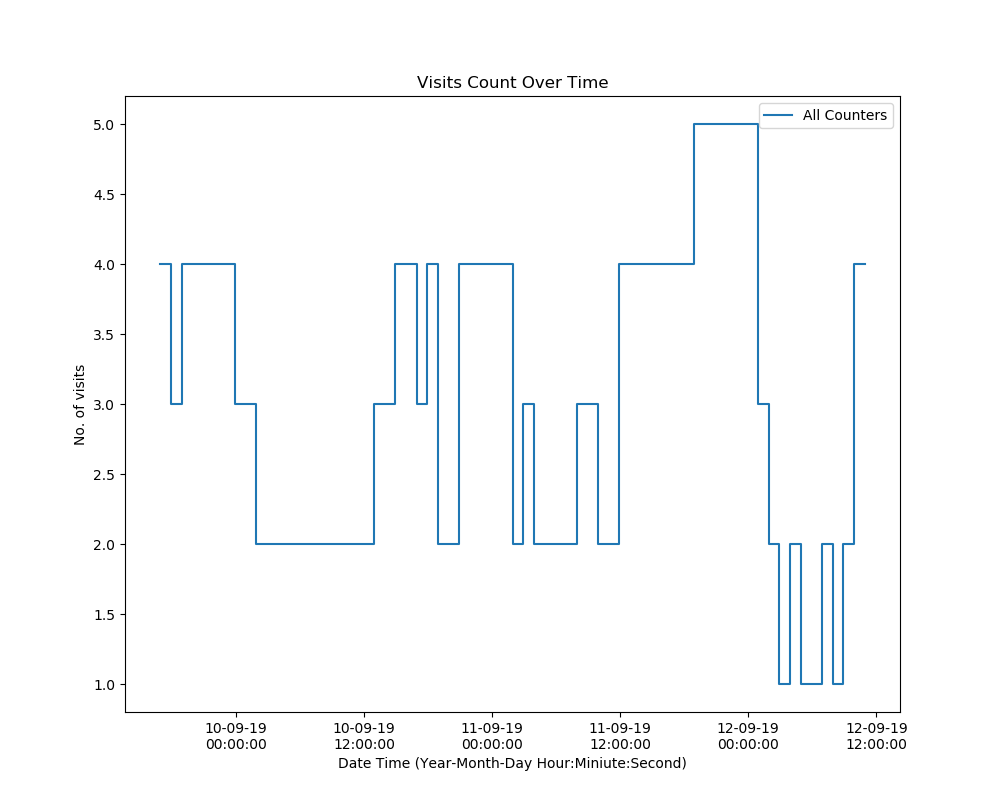
\includegraphics[width=225]{count_over_time.png}
    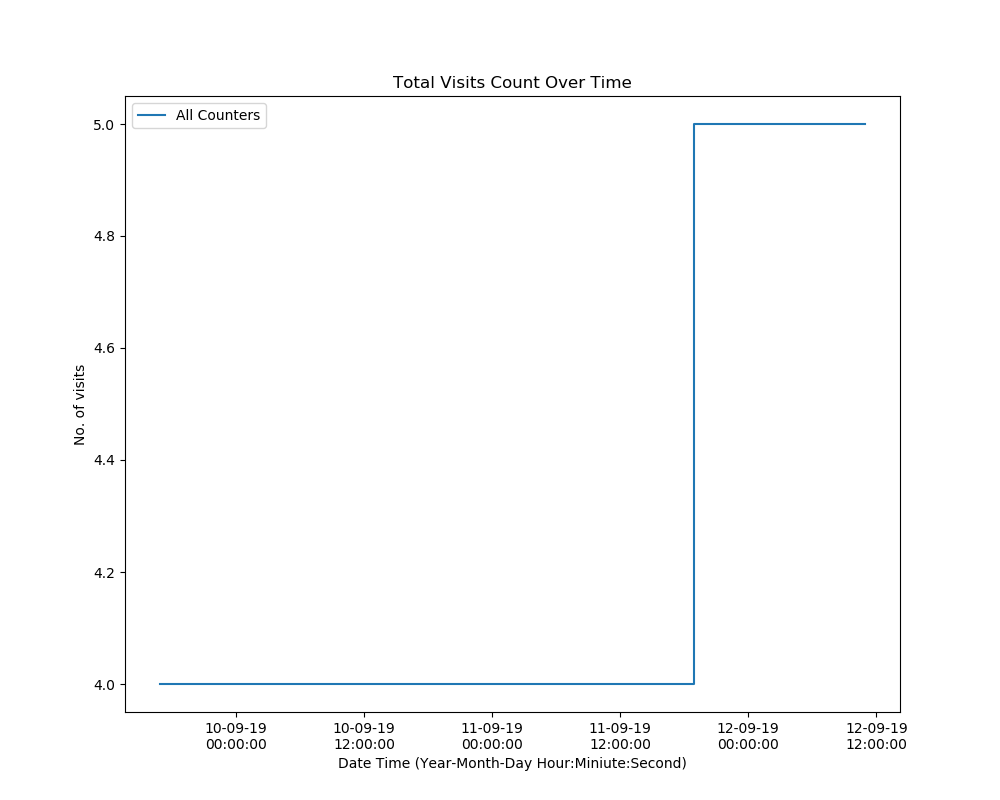
\includegraphics[width=225]{total_count_over_time.png}
    \caption{Counts & Total Counts Over Time : these graphs show us the count per hour of mobile devices. In the count over time graph, peak hours can be seen to be '11-09-2019 18:00:00' and '12-09-2019 00:00:00' at 5 mobile devices. }
    \label{fig:CountOverTime}
\end{figure}{} \\
As the counter graphs were completed the next graph to be created was the 'RSSI/Distance over time' graph, however, to complete this a formula would need to be applied to calculate the distance from the RSSI. This formula is:\cite{RSSItoDistance} \\
\begin{center}
   $Distance = 10^{((Received Power-RSSI)/N)}$ 
\end{center}
Where 'Measured Power' is the RSSI value at one meter and is the environmental power, which changes depending on the environment. This environmental power is usually between 2-4, however, the 'Indoor tracking using RSSI' report\cite{IndoorTrackingRSSI} uses a method to calculate this value depending on the environmental. However, in the code at the current moment of time is set to 2 as default.  This was used to create the 3rd graph in Table \ref{tab:g_sql_queries} using the methods 'rssi\_to\_distance\_graph()' and 'convert\_rssi\_to\_distance()', this graph was plotted by calculating the Distance vs RSSI ratio between -1 to -100 and was then plotted. The code and graph can be seen in Figure \ref{fig:rssiToDistance} and \ref{fig:rssiToDistanceGraph}. 
\begin{figure}[h!]
    \centering
    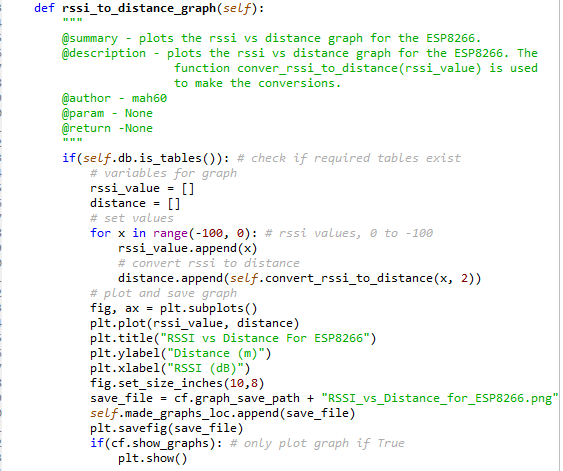
\includegraphics[width=175]{rssiToDistance_1.PNG}
    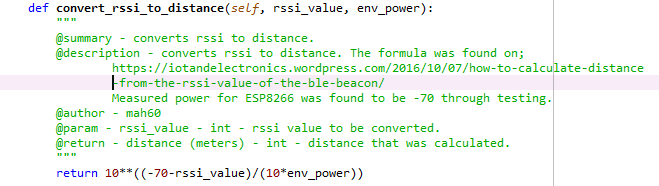
\includegraphics[width=175]{rssiToDistance_2.PNG}
    \caption{rssi\_to\_distance\_graph() & convert\_rssi\_to\_distance() Code}
    \label{fig:rssiToDistance}
\end{figure} \\
\clearpage
\begin{figure}[h!]
    \centering
    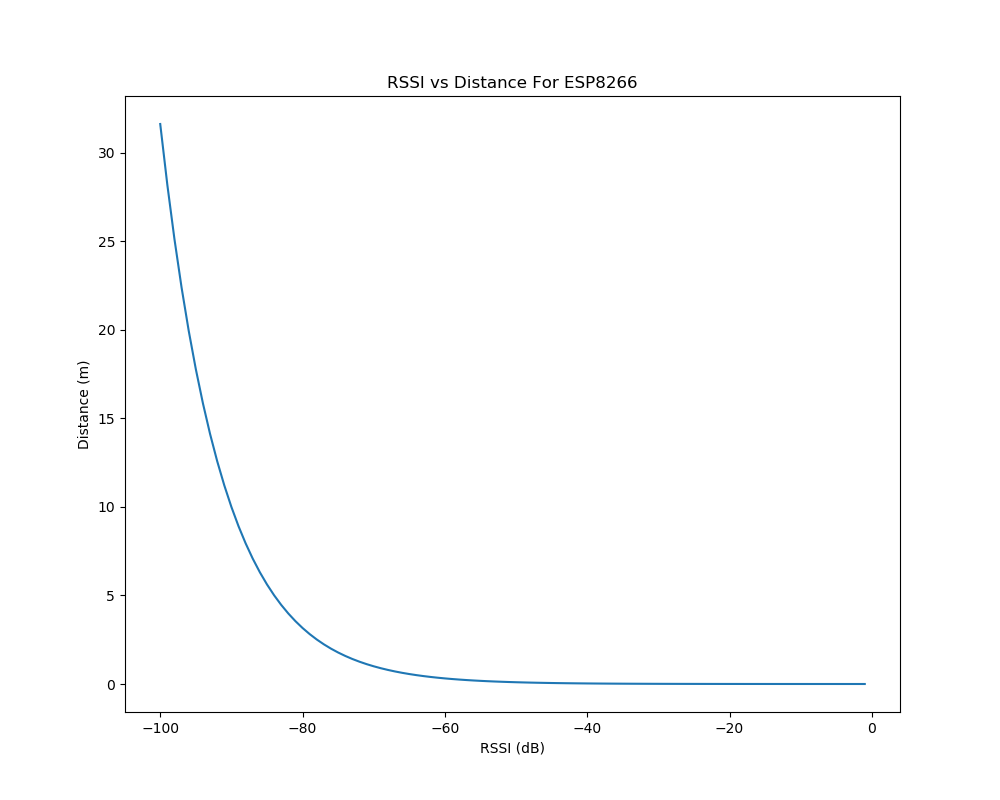
\includegraphics[width=200]{RSSI_vs_Distance_for_ESP8266.png}
    \caption{RSSI vs Distance Graph : The RSSI to distance conversion follows a inverse logarithmic curve.}
    \label{fig:rssiToDistanceGraph}
\end{figure} \\

The received power was calculated by conducting an experiment that had the WiFi Counter record a specific device which was playing a video at 1 meter. The average RSSI for a five minute time frame was then recorded. This test was conducted 10 times and then an overall average was calculated. This experiment can be seen in Table \ref{tab:RSSIoverTime} and the average RSSI value at one metre can be seen to be -70. The variation is between -67 and -72 within these results. Tests 1 and 2 hold less weight to the final value as no video was playing during the test, which means there will be less recordings of the device in the time frame as it was idol.\\ 
\begin{table}[h!]
    \centering
    \begin{tabular}{|c|c|}
    \hline
         Test & Average RSSI (dBm)\\
    \hline
        1 & -78.00 \\
        2 & -77.33 \\
        3 & -69.31 \\
        4 & -71.07 \\
        5 & -67.04 \\
        6 & -70.09 \\
        7 & -72.05 \\
        8 & -68.49 \\
        9 & -71.70 \\
        10 & -72.54 \\
    \hline
    \end{tabular}
    \caption{RSSI Over Time Experiment}
    \label{tab:RSSIoverTime}
\end{table} \newline
Once this formula and values were implemented into the code it was then easier to construct a graph that would tell us the distance/RSSI value over time for a specific device. This was then completed by using the query seen for graph 4 in Table \ref{tab:g_sql_queries}. The values returned from these queries were then sorted and if the distance boolean was set to true then a graph of distance over time would be produced instead. These can be seen in Figure \ref{fig:rssiDistanceOverTime} and \ref{fig:rssiToDistance} for the code. \\ \newline
\clearpage
\begin{figure}[h!]
    \centering
    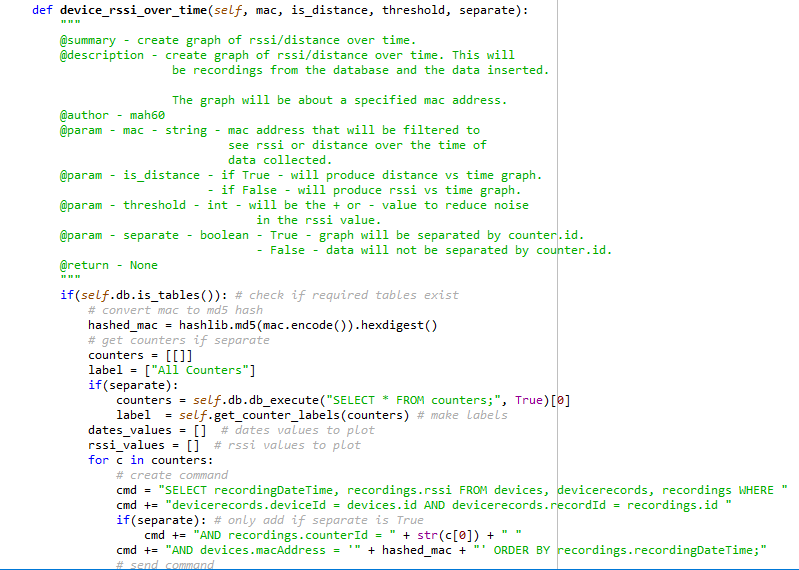
\includegraphics[width=175]{distance_rssi_over_time_1.PNG}
    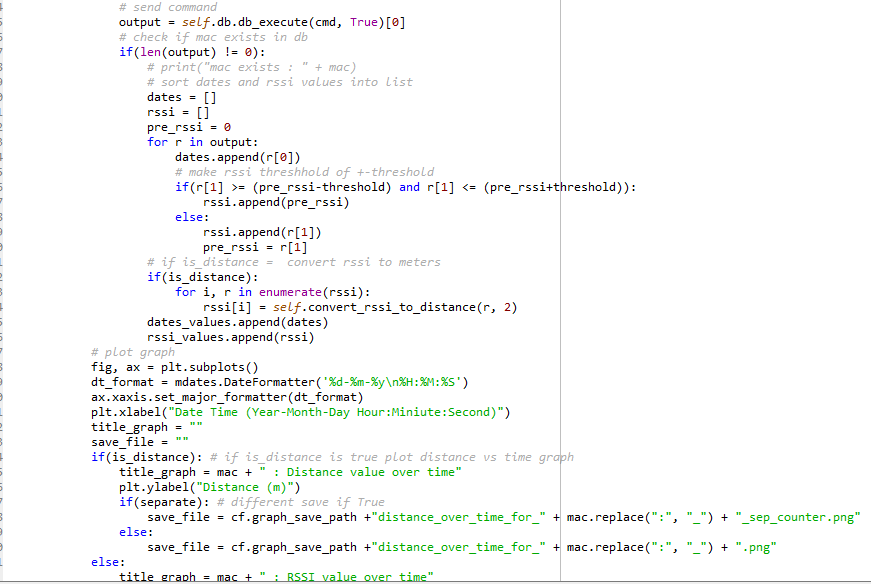
\includegraphics[width=175]{distance_rssi_over_time_2.PNG}
    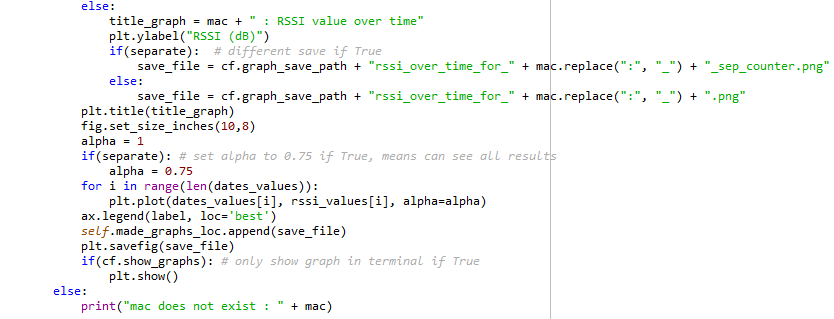
\includegraphics[width=175]{distance_rssi_over_time_3.PNG}
    \caption{device\_rssi\_over\_time() Code}
    \label{fig:rssiToDistance}
\end{figure} \\
\begin{figure}[h!]
    \centering
    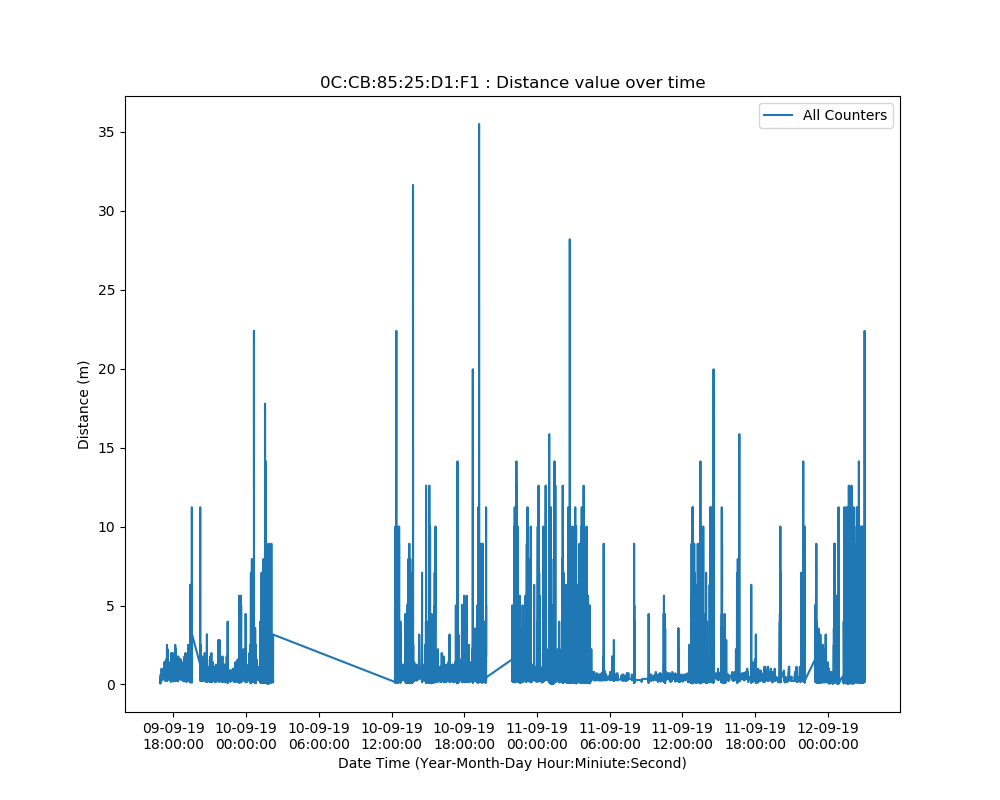
\includegraphics[width=225]{distance_over_time_for_0C_CB_85_25_D1_F1.png}
    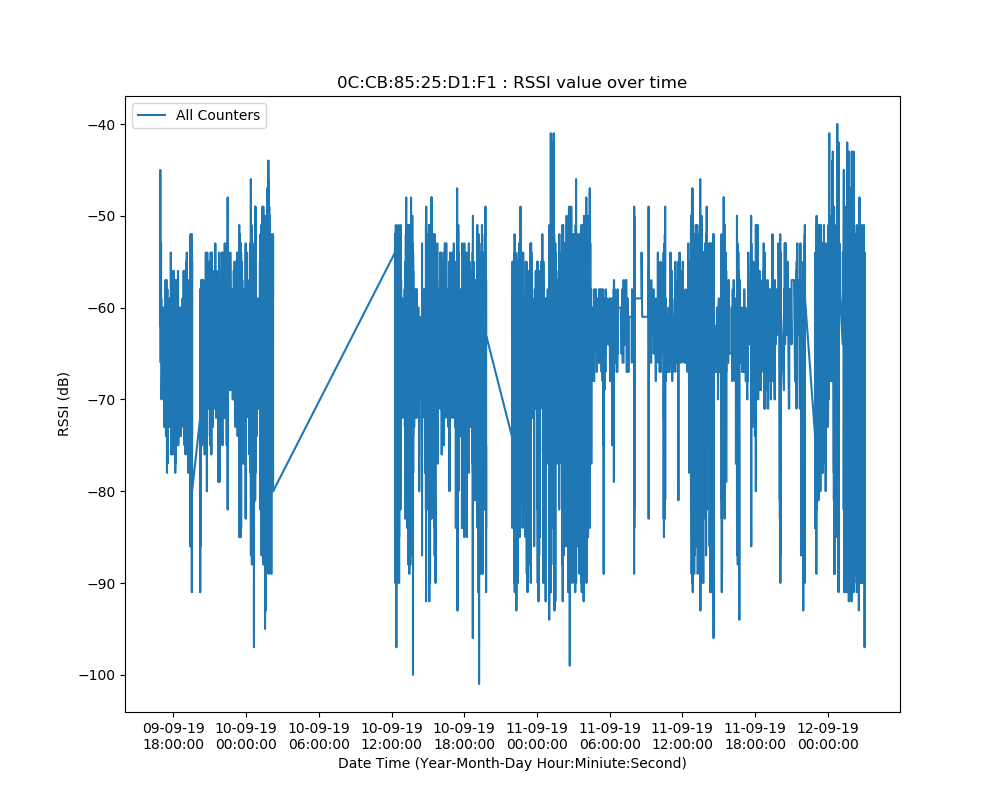
\includegraphics[width=225]{rssi_over_time_for_0C_CB_85_25_D1_F1.png}
    \caption{0C:CB:85:25:D1:F1 Distance/RSSI Over Time Graph :  this graphs show the inaccuracy of the ESP8266 as RSSI value ranges between -90 and -50. Therefore, the device is either moving around or the error rate is high due to the amount of noise in the surrounding area. The device is seen to be undetected between '10-09-2019 3:00:00' and '10-09-2019 12:00:00'.}
    \label{fig:rssiDistanceOverTime}
\end{figure} \\
The next graph to develop was a histogram of dwelling time, this was done by using the SQL query for the 5th graph in Table \ref{tab:g_sql_queries} which would order the dataset by 'recordingDateTime'. This would allow the code to sort through the records from start to end time stamp. The dwelling time would be calculated by looping through each recording in date order, there is then a list called 'mac\_addresses' which would record what devices were seen, when first seen and last seen. This could be used to calculate the dwelling time once the device had not been seen for x amount of time (Timed out). This dwelling time would then be calculated by subtracting the start time by last seen time. This method was also applied once all records had been checked to ensure all dwelling times were accounted for until the end of the WiFi Counter session. The next task was to plot the histogram, the code for this method and graph can be seen in Figure \ref{fig:dwellingTime} and \ref{fig:histdwellingTime}.\\ \newline
\begin{figure}[h!]
    \centering
    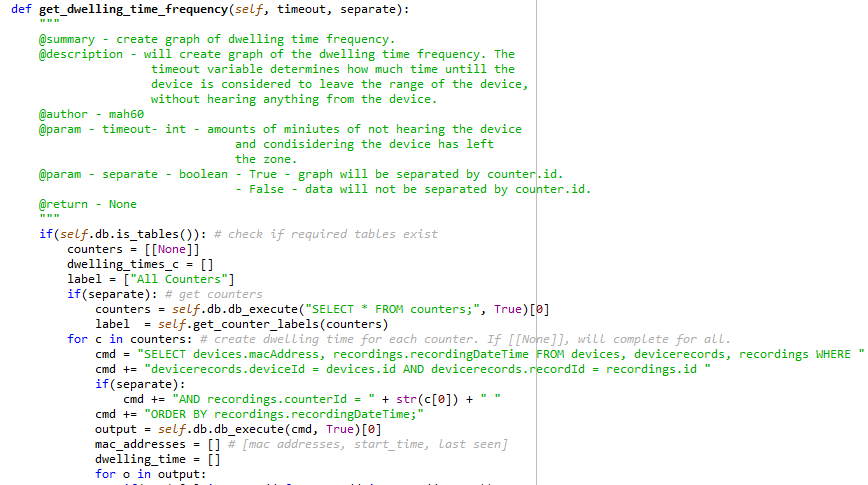
\includegraphics[width=200]{dwellingTime1.PNG}
    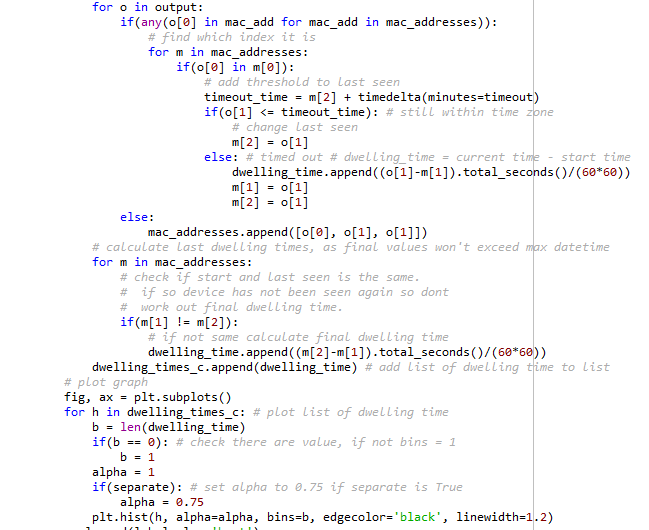
\includegraphics[width=200]{dwellingTime2.PNG}
    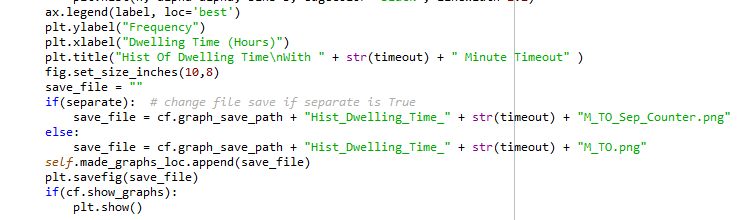
\includegraphics[width=200]{dwellingTime3.PNG}
    \caption{get\_dwelling\_time\_frequency() Code}
    \label{fig:dwellingTime}
\end{figure} \\ 
\begin{figure}[h!]
    \centering
    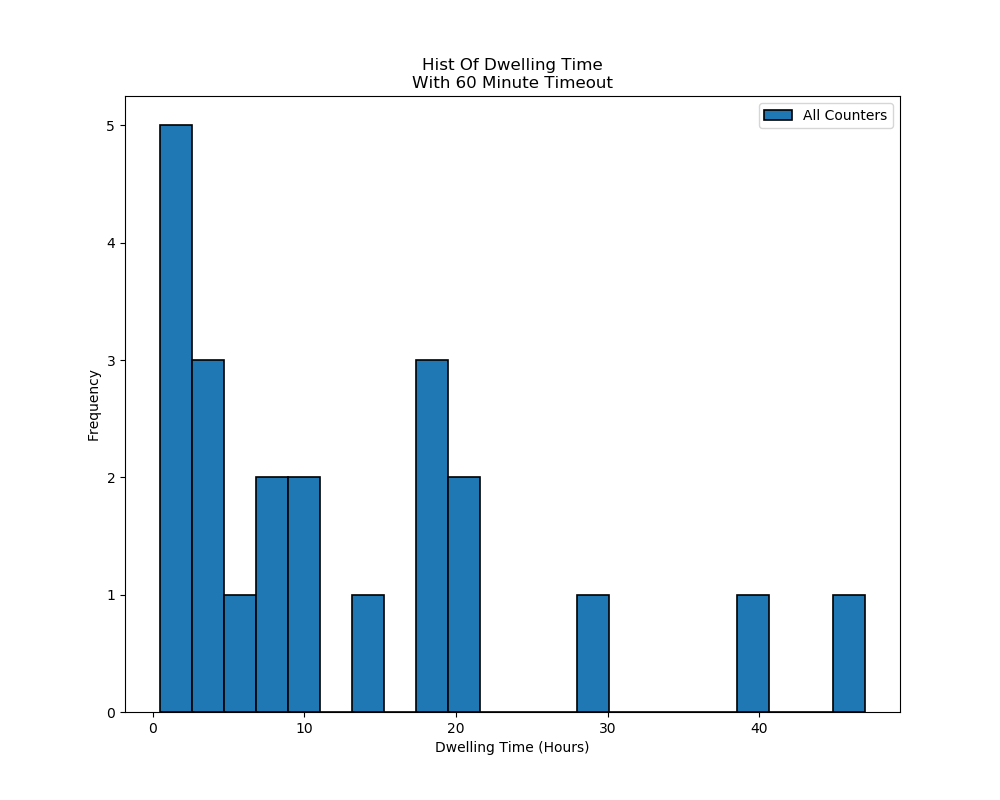
\includegraphics[width=200]{Hist_Dwelling_Time_60M_TO.png}
    \includegraphics[width=200]{Hist_Dwelling_Time_30M_TO.png}
    \caption{Histogram Of Dwelling Time : shows the frequency's of dwelling times within the WiFi Counters with a x minute timeout. This timeout will alter the about of bins within the histogram as there are varying dwelling times.}
    \label{fig:histdwellingTime}
\end{figure} \\ 
The final graphs to develop was to create a sub type of each graph which would separate the plot by each WiFi Counter. This could be used to present where the most used locations were and which counters were producing the most useful data. To do this was simple as the SQL query shown in graph 6 for Table \ref{tab:g_sql_queries} needed to be inserted into the other graph queries after the 'FULL OUTER JOINS' were complete. Then each of the queries will only get the data for 'counter.id' given, this means that to separate the data by WiFi Counter you need to loop through each Counter from a "SELECT * FROM counters;" query. This is done for each graph and then the methods are rearranged to allow for multiple sets of data to be plotted to each graph. An example of this can be seen in Figure \ref{fig:sepbycountersgraphs}. A legend is also applied to show what colour represents what Counter.\\ \newline 
\clearpage
\begin{figure}[h!]
    \centering
    \includegraphics[width=200]{count_over_time_sep_counters.png}
    \includegraphics[width=200]{Hist_Dwelling_Time_60M_TO_Sep_Counter.png}
    \includegraphics[width=200]{rssi_over_time_for_0C_CB_85_25_D1_F1_sep_counter.png}
    \caption{Graphs Separated By WiFi Counters : These graphs tell us the same information as the original graphs. However, as they are now separated by WiFi Counter, you can use that information to learn which areas have highest peak hours or which counter picked up x device. }
    \label{fig:sepbycountersgraphs}
\end{figure}  \\
The final phase of the visualisation is to place the graphs created onto a handout pdf. This can be done by using the FPDF library\cite{FPDF}, which will be using PHP to write a style sheet for the document. This document uses a query that selects the start and end timestamp of recording, number of devices, number of counters and number of records. The graphs are then added to the pdf through a 'for' loop, a variable of save paths are used to collect the images. The code for this can be seen in Figure \ref{fig:sendPdfPlusHandout} and an example of the first two pages. \\ \newline
\clearpage
\begin{figure}[h!]
    \centering
    \includegraphics[width=200]{sendToPDF1.PNG}
    \includegraphics[width=200]{sendToPDF2.PNG}
    \includegraphics[width=150]{handout1.PNG}
     \includegraphics[width=150]{handout2.PNG}
    \caption{send\_graphs\_to\_pdf() Code & Handout}
    \label{fig:sendPdfPlusHandout}
\end{figure} \\ 
The final deliverable to create a device that will be used to research what data that can be gathered from mobile devices in different environments has been developed. This deliverable is a handout of different statistics and graphs to represent the data gathered by the WiFi Counters. These visualisations use queries that collect the data with efficient speed.
\clearpage
 
%-------------------------------------------------------------------------------------------------------
% Testing
%-------------------------------------------------------------------------------------------------------
\section{Testing}
The testing phase of the project is done to ensure that all parts of the product that were built worked as planned. The tests were planned in the earlier stages of development and were then executed during development. These tests will need to be executed anytime major changes are made to the code to ensure that the product was not broken by the modifications made. There were several different types of testing that were done throughout this project, which were:
\begin{itemize}
    \item Acceptance Tests\cite{AcceptTest} - to access the acceptability of the product produced and ensures that all requirements are complete. 
    \item Unit Tests\cite{UnitTest} -  tests the individual parts of the code. To ensure all methods and objects work as planned.
    \item Debugging - to identify and remove errors within the code. This was done by either using the Debug method or printing strings to see where the error is occurring.
    \item Stress testing - to test the amount of data a product can take. This could be the amount of time the product can run for or to evaluate how a device reacts to specific types of data.
\end{itemize}
These different tests can be seen in the appendix, is the Acceptance Testing document, which has a template and a completed test for the code completed at the end of the project. The acceptance testing will also be using the MySQL Workbench\cite{MySQLWorkbench} to ensure that the data importer has collected and processed the data correctly. In some of the acceptance test that were completed, they were registered as failed. Such as, being able to detect if two mobile devices belong to the same person. These requirements were not completed as they have lower priority to other objectives and due to time constraints of the project.
\\ \newline
The tests that were done in the WiFi Counters code were mainly debugging. This is because unit tests are created to access the quality of the code, whereas, if unit tests were performed on the WiFi Counter it would be to test the functionality of the code, as we want to test if the product will work for the purpose of its development\cite{UnitTestsESP8266}. Therefore, using acceptance testing and debugging will be done on the WiFi Counter to determine the practical use of the product. Then the unit tests were developed on the Data Processor to access quality of the code for methods that returned data and did not manipulate the database this was done using the library 'Unittest'\cite{unittest}.\\ \newline
The final tests that were completed were stress testing. This was to test if the WiFi Counter could run for a set period of time. The highest time was a week, which the product showed no issues with that were not already recognised. Another stress test would be if the Data Processor could handle the import from multiple devices and a dataset from over the week period. This test produced no issues as the results can be seen in the 'DataProcessor/reports' in the technical hand in. However, even though these tests were conducted the full extent of tests planned for the deliverables could not be completed. As the ethical clearance was cleared at such a late stage in the project no tests could be conducted with participant devices, other than my own and tests to look at what data can be collected in different environments were not completed.\\ \newline
In conclusion, the acceptance and unit tests are used to pick out errors within the code, to access the quality of the code. From these tests you can understand the areas of the product that has issues and then use the debugging techniques to find the location of the problem and fix it. The stress testing will access the performance of the final product and how much it can handle. The next step is to look at the results of the final product.
\clearpage
%-----------------------------------------------------------------------------
% Results
% ---------------------------------------------------------------------------
\section{Results}
The final product consisted of multiple components that will help to collect and process the data needed. These components were :  
\begin{enumerate}
    \item Database Architecture with Database Manager
    \item WiFi Counter
    \item Data Importer
    \item Data Processor with handout 
\end{enumerate}
The product produced can approximate the amount of visits to a certain area and produce statistical models about the dataset produced. These graphs can be seen throughout the visualisation section, from the testing that was conducted there were flaws found within the WiFi Counter and the Data Processor components. Which were : 
\begin{itemize}
    \item Soft WDT reset - Watchdog error\cite{SoftWDTReset}- The WiFi Counter resets itself when a piece of code is taking too long. 
    \item Importing data - The importing to data takes a few minutes to transfer the data from the text file to the database. This issue is suspected to be because of the formatting process to generate the different queries for the inserting data into the databases.
    \item Creating total count and count over time graph -  Gathering the data for this graph takes a long time. This is because a separate query is used for each hour between the max and minimum time of recording. This causes issues because for each query the database needs to be sorted to be within range of the date time values given.
\end{itemize}{}
These are the main issues found from the testing completed. They mainly involve the amount of time a task takes to complete, due to this there will need to be further research into reducing the time taken to collect and store data in the database. However, even though these issues exists the final product can be counted as a success as it completed almost all high priority tasks in the objectives table ( Table \ref{tab:obj} ). The only high priority task to not be completed is to test the product in different enviroments, a controlled environment with multiple mobile devices. This was due to the ethical problem that was discussed at the start of this chapter. \\ \newline
The graph produced by the final product all demonstrate valuable information about the surroundings of the WiFi Counters. The information that can be learned from the graphs produced about the WiFi Counter is that the RSSI to distance conversion rate is a inverse logarithmic graph. As seen in Figure \ref{fig:rssiToDistanceGraph}. The value of 1 meter is -70 dB then the range exponentially increases. This means the conversion get less accurate the further away the device is. The RSSI of a specific mobile device in Figure \ref{fig:rssiToDistance} is seen to be between -90 to -50 throughout the time period of the recording. This means the inaccuracy of the ESP8266 on RSSI varies between -90 and -50 dB, this could be because of the amount of noise produced by its surroundings. As WiFi signals will bounce off walls which will then change the final signal strength value and will have a high error rate. \\ \newline
The final product produced can be used within the first two use cases discussed in the introduction chapter, as the final product can be used to create a network of WiFi Counters to collect data over a small to large area. This data can then be processed to create useful visualisations for a event manager. To work out peak hours, total visits and dwelling times. However, the third and forth use case will require more research into RSSI to distance conversion.  This is because to make a functioning position tracking system, accurate distance measurements between devices will be required. The main issues is that the WiFi Counter will have to filter readings to MAC addresses that have given consent to collect information on their devices due to the ethical clearance. 
\clearpage
%-------------------------------------------------------------------------------------------------------
% Future Development And Maintenance
%-------------------------------------------------------------------------------------------------------
\chapter{Future Development}
Future work for this project involves improving the product that was built through research and improving the quality of the code. There are several different jobs that can be done for future development or tasks. This is because of the potential of what this type of data collection can be used for is high and due to the problem with the ethical clearance some tasks were not completed in time. The future development that can be done are:
\begin{enumerate}
    \item Develop a dynamic network which will record data via a WiFi Connection, every x time period. 
    \item Research into methods to improve the accuracy of RSSI in different environments.
    \item Test the WiFi Counter in multiple environments. See how the data varies depending on its surroundings.
    \item Complete expected and potential objectives that were not completed in Table \ref{tab:obj}. For example, to be able to check if multiple devices belong to one person. 
    \item Use BCP utility\cite{BCP} instead of 'Insert many' query to import data to increase the speed of imports.
    \item Use CSV file instead of text file to record data on the WiFi Counter or improve structure of recorded data on the WiFi Counter. To reduce the amount of formatting needed to be done. 
\end{enumerate}
Additionally, the future work that is valuable completed are use case 3 and 4, which were to create a path tracking application and rerouting application. The final product has began these stages by being able to collect the RSSI value, this variable is then used to convert RSSI to distance. This can be seen in the Development chapter for the visualisations section. However, further research will need to be completed to improve the accuracy of this value either by modifying the hardware or understand how the environment surrounding the WiFi Counter effects the RSSI value. The information gathered from the TFL WiFi tracking\cite{GizmodoLondon} and Indoor location tracking\cite{IndoorTrackingRSSI} literature can help support the development of this. A method to counter the feedback loop mentioned in the TFL WiFi tracking\cite{GizmodoLondon} could be to use the D* searching algorithm\cite{Dstar} for artificial intelligence to alter the weights of the different routes that could be taken. This will vary the routes more efficiently and reduce the chance of the routes becoming overloaded by traffic. \\ \newline
There are different areas in which the data collected could be used for, some more suitable than others. However, the potential in which this research could be used for is great. As the data collected could improve migration between two different locations and support health systems, as shown by the 'WiFi Tracking using Arduino WiFi Shield' report\cite{ProtrackingArduino}, the system has the potential to gather improved position tracking to GPS inside a building .  
%-------------------------------------------------------------------------------------------------------
% Critical Evaluation
%-------------------------------------------------------------------------------------------------------
\chapter{Critical Evaluation}
The product build during the project could successfully collect and present data about an individual mobile devices. This was done by creating a device that would collect data by intercepting packets being sent through WiFi, using promiscuous mode\cite{Promiscuous_mode}. The product that was built was to be used in the following use cases: 
\begin{enumerate}
    \item Small Area Visit Counter
    \item Medium Area Visit Counter
    \item Path Tracking Application
    \item Rerouting Application
\end{enumerate}
During the projects lifespan, it has been shown that the information gathered about the ethics in the literature review was found to be correct. There were several problems that occured during the project to try and gain ethical clearance to complete the testing phase with participants. The best results would be to gather information from all mobile devices in the WiFi Counters surroundings. Whereas, the actual results for the final product can only gather data from the participant devices that have given consent to collect the data. The main issue that the ethical clearance brought to the project was that it took a long time to sort out and find a suitable manner to conduct testing in. Due to this issue the device that was developed was only tested by using the developers mobile devices to ensure the product worked as planned, meaning the product could struggle with collecting data on multiple devices. The ethical clearance could have been handled better to reduce the amount of delays and issues that were seen throughout this project. This would have been done by truly understanding how delicate the data being collected was under the GDPR\cite{GDPR} as they were seen to be personal data and fully understanding the research that was conducted in the literature review for 'Smart Bins'\cite{Smart_bins} and 'TFL WiFi tracking'\cite{GizmodoLondon} and learning from their mistakes. These projects showed a method to gain ethical clearance and the issues that came with collecting the data. The alternative approach that should have been taken was to initially state that the device would only be used on mobile devices that have given permission for collecting their data. Then further research would need to be conducted to allow use of the WiFi Counter without permission or alternatively look into scenarios that will ask a user for permission, for example, tracking an employee around the companies building in case of an emergency and then the device can be activated to alert the position of where the employee is to the appropriate authorities. \\ \newline
A method to counter the ethical clearance problem that could have been implemented would have been to build mobile devices through the use of the ESP8266 MicroControllers. Then once they were created this method could have allowed for the product to be tested in controlled environments with multiple devices without the use of any participants. However, this method would have been more financially expensive but overall would of provided a method to test the final product under ethical circumstances.\\ \newline
 The objectives in Table \ref{tab:obj} represent the different tasks that had to be completed throughout the projects lifespan. These objectives were split between whether they were seen as Expected, Potential or Future work and were all given priority levels for what order the objectives needed to be completed in. The objectives helped to organise the project and allowed the project to follow a certain flow to allow for key objectives to be completed. As issues occured throughout the project, it could then be reorganised to enforce that almost all high priority tasks were completed. However, the main high priority objectives that were not completed was to test the WiFi Counter in different environments. This is due to the ethical clearance issue and meant the device was mainly tested within the developers house and not in different environments as the clearance to conduct tests in different environments was not given. Nevertheless, possible future work that could be conducted to improve the product can be seen within the objectives table. As well, in the future work sections there are examples of where the project could be taken.\\ \newline 
 The objectives table allowed for the project to be completed and ensured that all high priority tasks were completed. However, this meant that little research was completed to look into the other objectives, such as, telling if a participant had multiple mobile devices on them. The process of using feature driven development (FDD) helped to support the project, as each component was completed, the next task would begin and designed around the components already made. Meaning a order was given the products production. However, further development should of been done to the previous components as the project progressed to complete objectives of lower priority. An alternative approach would of been to use a methodology like Scrum\cite{Scrum} to access the progress of the project every sprint and what could be done to improve the project. This method will also allow for priority levels to change throughout the project as problems occur or different objectives become more or less important. \\ \newline 
The WiFi Counter was capable of completing the first two use cases, as a single WiFi Counter can be used to record data in areas of varying sizes, depending on how many WiFi Counters are used. This was done by collecting the SD cards from the WiFi Counters and then uploading the data collected to the database that was designed to store and handle the data collected efficiently. The main problem with uploading the data from the SD card is that the formatting takes a few minutes due to the amount of records. This could be reduced by reformatting how the data is saved to the text file, to make the transactions between the text file and the database smoother, this could be done by using a CSV file instead. Another feature that could reduce the formatting time, would be to add a real time clock to the ESP8266. This would allow for the time of recording to be registered without the use of the additional millis variable. However, once the data was collected and stored inside the database the processing is efficient and produced several statistics and visualisations that represent the potential of what information can be learnt from the data gathered. This information is then sent to a PDF handout that can be sent to managers to show them the statistics of how many people visited the event or area and for how long. These can be seen in Figure \ref{fig:exampleGraphs} and \ref{fig:sendPdfPlusHandout}. The data currently gathered can be seen to be reliable when recording what mobile devices are near by, however, as the distance to RSSI conversion rate is not accurate due to the noise for the RSSI value. It becomes harder to create a range of where to filter out devices from. As the range will need to be the variation of RSSI in a particular device around the WiFi Counter. Although further investigations could be conducted to see what information can be gained from the data recorded and perhaps what additional data could be gathered from mobile devices using promiscuous mode or different tools. \\ \newline
The network of WiFi Counters is a cheap alternative to using a Arduino or Raspberry Pi. As to produce the device the Micro SD Card modules are £1 each and the ESP8266 are £3 each. This means a large amount of WiFi Counters can be built to create a network over a medium or large area. However, the final network that can be built from WiFi Counter will not be dynamic in uploading data to a server or database. Meaning all data will need to be collected in person. A potential task for future development is to make the network dynamic in uploading and analysis. Another, potential improvement would be to add a battery bank and container for the device to the WiFi Counter, to make the device portable around a range of environments. Alternative approaches such as using the Raspberry Pi\cite{RaspberryPi} should be looked into as the microcontroller may have improved accuracy on the ESP8266 that would deem for the change between the devices to be appropriate. This will depend if the requirements are wanting the device to be financially cheaper or more accurate. \\ \newline
The project lays out future development into the 'path tracking application' and 'rerouting application' use cases. The product could implement path tracking through the use of multiple WiFi Counters, to collect the information by either connecting the devices by mobile device or using the position tracking technique to calculate the path that the device takes.  This is because the research conducted began to look into converting RSSI to Distance, this research can be seen in visualisations in the development chapter . This can be seen in the graphs in Figure \ref{fig:rssiToDistanceGraph} and \ref{fig:rssiDistanceOverTime}, for RSSI to Distance and the Distance for a particular device over. Showing the potential of what information can be gained from using the product produced, however, further research will need to be completed to accurately estimate a persons location and the use of multiple WiFi Counters will be required for this task. The path tracking methods in the 'Indoor Location Tracking'\cite{IndoorTrackingRSSI} report discusses potential methods to track a mobile device. As well, as proven by the report and the results shown in Figure \ref{fig:rssiDistanceOverTime} the error rate is high when it comes to measuring distance using RSSI and the WiFi. This is due to the amount of noise in the surrounding areas as the signals will bounce off walls or other obstacles, therefore it becomes more difficult to gain an accurate value of the signal strength (RSSI).  As well, due to the nature of the RSSI to Distance formula that can be seen to be a inverse logarithmic curve in Figure \ref{fig:rssiToDistanceGraph} for the RSSI vs Distance graph. The conversion rate between RSSI to distance from this graph can be seen to be accurate till the received power of -70 is reached. However, once reached the conversion becomes less accurate as the value exponentially increases.\\ \newline
The potential that the device being built could be expanded out into multiple different areas, the initial stages of this project was to design a product that could approximate the amount visitors in an area. Whereas, the data learned can be used to create a device that would help transportation or have improved position accuracy within a building to GPS, which could be used to find employees in an emergency.  This was completed by using the WiFi Counter to record when signals sent off by mobile devices were intercepted. The final product can completes these tasks, however, a method will need to be applied to tell if a person is holding multiple devices and whether the data being recorded is from a mobile device or a stationary one. As there may be a set of devices which do not move in the dataset, which will be pointless to record as the device was made to record the number of visitors. This could be done by calibrating the device to remove any devices that seem to be stationary over the recording time. As the graph about RSSI over time in Figure \ref{fig:rssiDistanceOverTime}, you can see that variation in RSSI is the same throughout the recording time. This means the device is stationary. Nevertheless, the data recorded can be analysed to produce statistics about the dataset. Such as, the peaks hours, dwelling time and the total amount of visits. This data can then be translated to different statistical models and finally into a pdf handout. However, with further research into the product and its benefits the device could be used in multiple areas to produce useful data for multiple companies about the consumers that wander their events or stores. To understand the nature of the consumer, the most used routes, travel times, an example of this can be seen in TFL WiFi Tracking\cite{GizmodoLondon} as they develop a network that tracks Oyster card members across the London Underground. Whereas, this product would be a cheaper alternative that produces familiar information.
%-------------------------------------------------------------------------------------------------------
% Conclusion
%-------------------------------------------------------------------------------------------------------
\chapter{Conclusion}

%-------------------------- 
In conclusion, the final product that was built can collect data on the number of visitors within its surroundings through the use of mobile devices and then produce graphs and statistics about the data recorded. This was done by developing the WiFi Counter and Data Processor, that would collect and analyse the dataset produced through intercepting mobile devices packages. The WiFi Counter can be used by itself or with multiple other WiFi Counters to form a network of data collectors over a varying sizes of areas. However, the text files that were produced by the WiFi Counters will need to be collected in person and then uploaded to the Data Processor through the Config file. The output from the Data Processor will be a PDF handout that will contain statistics and visualisations based on the variables set within the Config file. \\ \newline
There are issues with the final product, however, with time these problems can be countered and developed to further improve the device. This will be seen as the network that will be built is not dynamic and the final product has yet to be tested in multiple environments.  However, these issues can be fixed by uploading the data recorded over WiFi during run time and working on gaining permission to test the device in different controlled environments. There are also other objectives that need to be completed in Table \ref{tab:obj}, as well as other tasks that could be implemented to improve the product. An example of this would be to improve the formatting system for transferring data between a text file and the database in the Data Processor or to use BCP utilitly\cite{BCP} to import data. \\ \newline
The major issue that was found throughout the projects lifespan was gaining ethical clearance. This was not completed till the late stages of the project. Therefore, the testing which could have been completed for different environments was not finished. This means that experimentation in different environments had to be pushed to future development. However, the main principles of the project were successful, this was to create the WiFi Counter that was then used to collect the data from individual mobile devices. Then to produce a report of what information can be gathered from mobile devices, which can be seen in Figure \ref{fig:exampleGraphs} and \ref{fig:sendPdfPlusHandout} as a handout of statistics and visualisations. The graphs show the total amount of visits over time, peak hours and dwelling times, then can be separated by WiFi Counters to see where people visited and stayed over the course of their encounter with the WiFi Counters. As well, the initial research into looking into position tracking was complete, however, further research will need to be conducted to improve the accuracy of RSSI to distance conversion. \\ \newline
The product that was built can successfully approximate the amount of people within an area. Although, research and development into other data that could be learnt from the dataset would improved the richness of what information could be learnt from the recordings. Even though this was true further development should be conducted to implement the device for different tasks and to improve the different features of the project. A challenge that will need to be look into how the personal data collected could be protected further and henceforth gain ethical clearance to complete the testing on the product with different enviroments and multiple mobile devices. 
\clearpage

\chapter{Version And Bibliography}
\begin{table}[h]
    \centering
    \begin{tabular}{c p{12cm} c}
    \hline
        Version & Description & Date  \\
    \hline \hline
        0.1.0 & Created the initial design for the document and created the introduction chapter. & 05/09/2019 \\
        0.1.1 & Wrote the literature review and proofread the document. & 08/08/2019 \\
        0.1.2 & Proofreading done for introduction and literature review. Wrote Development chapters
                    up to WiFi Counter implimentation. & 12/09/2019 \\
        0.1.3 & Wrote all the parts to the development and implimentation section. The ethics section is still not completed. &  15/09/2019\\
        0.1.4 & Proofread the development chapters and made edits. The figures and all citations were complete up to the end of the development chapter. & 18/09/2019\\
        0.1.5 & Wrote Testing and Future development section. & 20/09/2019 \\
        0.1.6 & Wrote Critical Evaluation and Conclusion. & 22/09/2019 \\
        0.1.7 & Proofread and edited, abstract, testing, future development, critical evaluation and the conclusion & 23/09/2019\\
        0.2.0 & Rephrasing document to sound better and to go along with new title. & 24/09/2019 \\
        0.3.0 & testing moved to development chapter and summary in development changed to results. Additional information added to critical evaluation to reflect final the project went & 26/09/2019 \\
        0.4.0 & Project methodology, acceptance testing template and test added to the appendix. & 26/09/2019 \\
        1.0.0 & Final report complete & 27/09/2019 \\
    \hline
    \end{tabular}
    \label{tab:my_label}
\end{table}{}
\begin{thebibliography}{9}

 \bibitem{Smart_bins}
    BBC News; Smart Bins News Report; 30/06/2019; \\
    \textit{https://www.bbc.co.uk/news/technology-23665490}\\
    
  \bibitem{GDPR}
    Manager Engine, Desktop Central; General Data Protection Act 2018; 05/09/2015
    \textit{https://www.manageengine.com/products/desktop-central/gdpr.html?network=g&device=\newline c&keyword=eu\%20gdpr&campaignid=1011560072&creative=238053253813&matchtype=e&adposition=\newline 1t1&placement=&adgroup=49007691279&targetid=kwd-297029345670&gclid=\newline
    Cj0KCQjw5MLrBRClARIsAPG0WGwunLNmdkXA7ldGHokGSpG-\newline
    peCMPYvTGTCnpENAyMXuioeWQG9Wm8AaAr-5EALw\_wcB}

  \bibitem{tomography}
   Wikipedia; Tomography Reconstruction; 05/09/2019;\\
   \textit{https://en.wikipedia.org/wiki/Tomographic\_reconstruction}\\
   
  \bibitem{RSSI}
  NetSpot Pro; RSSI; 05/09/2019; \\
  \textit{https://www.netspotapp.com/what-is-rssi-level.html} \\
    
\bibitem{SmartBins2}
   Quartz; Smart Bins Technology; 07/09/2019;\\
   \textit{https://qz.com/112873/this-recycling-bin-is-following-you/} \\
   
 \bibitem{ProtrackingArduino}
    Western Michigan University; Nathan Conrad; Position Tracking using wifi; 07/09/2019; \\
   \textit{https://pdfs.semanticscholar.org/c369/f4ea8cf81b14e445ac45fd4f2fa72d3f8c3f.pdf} \\

    \bibitem{GizmodoLondon}
    Gizmodo; London Underground Wifi Tracking; 07/09/2019; \\
    \textit{https://www.gizmodo.co.uk/2017/09/london-underground-wifi-tracking-heres-everything-we-learned-from-tfls-official-report/}\\
    
    \bibitem{IndoorTrackingRSSI}
    Indoor Location Tracking using Received Signal Strength Indicator; By Chuan-Chin Pu, Chuan-Hsian Pu, and Hoon-Jae LeeX at Taylor's University College, Dongseo University; 07/09/2019;
    \textit{http://cdn.intechweb.org/pdfs/13525.pdf?fbclid=IwAR14\_04kVjg3bRO\_uxkm3RnRwhmEhfMtVKL5\_xrwMcjyYXWcbpawTiJ-p08}
    
    \bibitem{WaterfallModel}
    ToolSQA; Waterfall Model; 17/09/2019;\\ 
    \textit{https://www.toolsqa.com/software-testing/waterfall-model/} \\
    
    \bibitem{Scrum}
    Scrum.org; Scrum; 17/09/2019;\\
    \textit{https://www.scrum.org/resources/what-is-scrum}\\
    
    \bibitem{FDD}
    Agile Modelling; Feature Driven Development; 17/09/2019; \\
    \textit{http://agilemodeling.com/essays/fdd.htm}
    
        \bibitem{Trello}
        Trello; Kanban Board; 12/09/2019; \\ 
        \textit{https://trello.com/en} \\
    
    \bibitem{Github}
    Github; Github Repository; 24/09/2019 \\
    \textit{https://github.com/}
    \bibitem{MacAddress1}
Privacy Company;  MAC address; 10/09/2019;
\textit{https://www.privacycompany.eu/en/what-does-the-gdpr-say-about-wifi-tracking/}\\
        
        \bibitem{MySQL}
        Guru99; MySQL ; 10/09/2019; \\
        \texttt{https://www.guru99.com/sql-vs-mysql.html}\\
        
        \bibitem{PostgreSQL}
        PostgreSQL ; 10/09/2019; \\
        \textit{https://www.postgresql.org/} \\
        
        \bibitem{SQLite}
        SQLite; 10/09/2019; \\
        \textit{https://www.sqlite.org/index.html}\\
        

        
        \bibitem{CAPTheorm}
        Towards Data Science; CAP Theorem; 12/09/2019; \\ 
        \textit{https://towardsdatascience.com/cap-theorem-and-distributed-database-management-systems-5c2be977950e} \\
        
        \bibitem{SQLvNoSQL}
        The Geek Stuff; SQL vs NoSQL; 12/09/2019;\\
        \textit{https://www.thegeekstuff.com/2014/01/sql-vs-nosql-db} \\
        
        \bibitem{Normalization}
        Study Tonight; Normalization; 12/09/2019; \\
        \textit{https://www.studytonight.com/dbms/database-normalization.php} \\
        
        \bibitem{MySQLWorkbench}
        MySQL; MySQL Workbench; 12/09/2019; \\
        \textit{https://www.mysql.com/products/workbench/} \\
        
        \bibitem{PostSQLvsMySQL}
        2nd Quadrant PostgreSQL; PostgreSQL vs MySQL; 12/09/2019; \\
        \textit{https://www.2ndquadrant.com/en/postgresql/postgresql-vs-mysql/} \\
        
        \bibitem{AduinoUno}
        Farnell; Arduino Uno; 12/09/2019; \\
        \textit{https://www.farnell.com/datasheets/1682209.pdf} \\
        
        \bibitem{RaspberryPi}
        Pololu; Raspberry Pi Model B, Revision B; 12/09/2019; \\
        \textit{https://www.pololu.com/product/2750}
        
        \bibitem{ESP8266}
        Wikipedia; ESP8266; 12/09/2019; \\
        \textit{https://en.wikipedia.org/wiki/ESP8266} \\
        
        \bibitem{ArdinoIDE}
        Arduino; Arduino IDE ; 12/09/2019; \\
        \textit{https://www.arduino.cc/en/main/software} \\
        
        \bibitem{Python}
        Python Software Foundation; Python; 12/09/2019; \\
        \textit{https://www.python.org/}\\
        
        \bibitem{Promiscuous_mode}
        Tech Target Search Security; Promiscuos Mode; 12/09/2019;\\ 
        \textit{https://searchsecurity.techtarget.com/definition/promiscuous-mode} \\
        
        \bibitem{SPIFF}
        Tttapa Github; SPIFFs; 12/09/2019; \\
        \textit{https://tttapa.github.io/ESP8266/Chap11\%20-\%20SPIFFS.html} \\
        
        \bibitem{SoftWDTReset}
        ESP8266 Arduino Core; Soft WDT Reset; 12/09/2019; \\
        \textit{https://arduino-esp8266.readthedocs.io/en/latest/faq/a02-my-esp-crashes.html} \\
        
        \bibitem{String}
        Majenko Technologies; The Evil of Ardino Strings; 13/09/2019; \\
        \textit{https://hackingmajenkoblog.wordpress.com/2016/02/04/the-evils-of-arduino-strings/}\\
        
        \bibitem{promiscuous_mode}
        Łukasz Podkalicki; ESP8266-WiFi Sniffer; 13/09/2019; \\
        \textit{https://blog.podkalicki.com/esp8266-wifi-sniffer/} \\
        
        \bibitem{activate_promiscous_mode}
        EspressIf;  Wi-Fi Library; 17/09/2019;\\
        \textit{https://docs.espressif.com/projects/esp-idf/en/latest/api-reference/network/esp_wifi.html}
        
        \bibitem{getCurrentTime}
        kaefert; Github; Get Timestamp; 13/09/2019;\\
        \textit{https://github.com/arduino-libraries/NTPClient/issues/36} \\

        \bibitem{NTPClient}
        Github; NTPClient; 13/09/2019; \\ 
        \textit{https://github.com/arduino-libraries/NTPClient} \\
        
        \bibitem{itoa}
        Adruino; itoa; 13/09/2019; \\
        \textit{https://playground.arduino.cc/Code/PrintingNumbers/} \\
        
        \bibitem{millis}
        Arduino; Millis; 13/09/2019; \\
        \textit{https://www.arduino.cc/reference/en/language/functions/time/millis/} \\
        
        \bibitem{wifMACaddress}
        Arduino; WiFi MAC address; 13/09/2019; \\
        \textit{https://www.arduino.cc/en/Reference/WiFiMACAddress} \\
        
        \bibitem{MD5}
        TechTarget; SearchSecurity; MD5 hash; 17/09/2019; \\
        \textit{https://searchsecurity.techtarget.com/definition/MD5}
        
        \bibitem{MD5Builder}
        Github ESP8266; MD5Builder; 13/09/2019; \\
        \textit{https://github.com/esp8266/Arduino/blob/master/cores/esp8266/MD5Builder.cpp}\\
        
        \bibitem{AESEncryption}
        Github; Arduino-Crypto; 13/09/2019; \\
        \textit{https://www.c-sharpcorner.com/article/what-is-encryptiondecryption-and-how-it-is-used-in-asp-net/}\\ 
        
        \bibitem{SD}
        Github ESP8266; SD library; 13/09/2019; \\
        \textit{https://github.com/esp8266/Arduino/tree/master/libraries/SD}\\
        
        \bibitem{SPI}
        NodeMCU; SPI documentation; 13/09/2019;\\
        \textit{https://nodemcu.readthedocs.io/en/master/modules/spi/} \\
        
        \bibitem{insertRecords}
        RedGate Hub; Eugene Philipov; Insert vs Insert many; 13/09/2019; \\
        \textit{https://www.red-gate.com/simple-talk/sql/performance/comparing-multiple-rows-insert-vs-single-row-insert-with-three-data-load-methods/} \\
        
        \bibitem{BCP}
        Microsoft SQL Docs; DCP utility; 13/09/2019; \\
        \textit{https://docs.microsoft.com/en-us/sql/tools/bcp-utility?view=sql-server-2017} \\
        
        \bibitem{bcpy}
        Python Software Foundation; bcpy library; 13/09/2019; \\
        \textit{https://pypi.org/project/bcpy/} \\
        
        \bibitem{hashlib}
        Python Software Foundation; Hashlib library; 17/09/2019; \\
        \textit{https://docs.python.org/3.5/library/hashlib.html} \\
        
        \bibitem{matplotlib}
        Matplotlib; Matplotlib library; 17/09/2019;\\
        \textit{https://matplotlib.org/}\\ 
        
        \bibitem{FPDF}
        FPDF; FPDF libray; 17/09/2019; \\
        \textit{http://www.fpdf.org/} \\
        
        \bibitem{Joins}
        W3School; SQL Joins; 17/09/2019; \\
        \textit{https://www.w3schools.com/sql/sql\_join.asp} \\
        
        \bibitem{selecctOpt}
        DZOne;  Francis Ndungu; Optimize SQL Queries; 14/09/2019; \\ 
        \textit{https://dzone.com/articles/how-to-optimize-mysql-queries-for-speed-and-perfor}\\
        
        \bibitem{RSSItoDistance}
         iotbymukund; iotandelectronics; RSSI to Distance; 15/09/2019;\\ 
         \textit{https://iotandelectronics.wordpress.com/2016/10/07/how-to-calculate-distance-from-the-rssi-value-of-the-ble-beacon/} \\
         
         \bibitem{UnitTestsESP8266}
         Stack Overflow; Iron Savior; Unit Tests on Arduino; 18/09/2019;\\
         \textit{https://stackoverflow.com/questions/780819/how-can-i-unit-test-arduino-code} \\
         
         \bibitem{Dstar}
         Dave Ferguson & Anthony Stentz; Carnegie Mellon University; The Field D* Algorithm for Improved Path Planning and Replanning in Uniform and Non-Uniform Cost Environments; 21/09/2019; \\
         \textit{https://pdfs.semanticscholar.org/58f3/bc8c12ee8df30b3e9564fdd071e729408653.pdf}\\
         
         \bibitem{AcceptTest}
         Software Testing Fundamentals; Acceptance Testing; 21/09/2019; \\
         \textit{http://softwaretestingfundamentals.com/acceptance-testing/}\\
         
         
         \bibitem{UnitTest}
         Software Testing Fundamentals; Unit Testing; 21/09/2019; \\
         \textit{http://softwaretestingfundamentals.com/unit-testing/}\\
         
         \bibitem{unittest}
         Python Software Foundation; Unittest Library; 21/09/2019; \\
         \textit{https://docs.python.org/2/library/unittest.html} \\
         
\end{thebibliography}

\chapter{Appendix}
%-------------------------------------------------------------------------------------------------------
% Project Methodology
%-------------------------------------------------------------------------------------------------------
\section{Project Methodology}
Project methodology is a key part to any project in that it defines the structure and organisation within the project. The method that is taken helps to decide how flexible the project time frame is and ensures that certain standards of work are kept throughout the time frame of the project to reduce the possibility of the final product being delayed. There are two types of methodologies that can be used throughout the project which are 'traditional' or 'agile'. Traditional is more focused towards having fixed stages throughout the project for deadlines and the work is completed in a fixed order. This can be seen in the Waterfall method\cite{WaterfallModel}. Whereas, agile focuses on being flexible and adaptable throughout development to ensure that if there are any delays in any of the tasks then the plan can be modified to best suit the current situation. This can be seen in Scrum\cite{Scrum}  and Feature Driven Development (FDD)\cite{FDD}. Therefore, the first task that had to be done before beginning this project was to decide which one of these models would be used to organise the project. \\ \newline
Overall, the decision of what methodology to take was an 'agile' approach, as this method allows for more flexibility throughout the project. The reason 'traditional' methods such as  the Waterfall model would not be useful for the project is purely due to the fact that once you reach the next stage of the project it is then very hard to backtrack to a previous stage in the development process. This is due to if you backtrack all the tasks then they will have to be checked again, further delaying the project and there are no deliverables till the late stages of the project. \\ \newline
Subsequently, this means an agile methodology is best to take throughout this project. The methodology that will be used is FDD. This is because as the project is already split into use cases and objectives, these can be used as the features during this project. A set of tasks will be set at the start of each week, which will be based around the use cases and objectives. Then after that week has been completed the work will be reviewed and the following weeks tasks will be assigned based on the previous weeks work. This methodology will ensure that the project is following a specific structure, while also staying flexible to any changes throughout the project development.\\ \newline
Finally, three additional methods were applied to ensure the project kept on track and up to standard. These were:
\begin{itemize}
   \item Kanban Boards - made on Trello\cite{Trello} and are there to help support the project by creating a ToDo list with priorities for the week. An example of this can be seen in Figure \ref{fig:kanban board}.
    \item Version Control - this is where each document will have a version number and documentation to state what was altered in that version. The version control will also be enforced by the GitHub repository\cite{Github}. This will allow for backtracking the code to an earlier version if required.
    \item Backups - this is where on a weekly basis the items developed are uploaded to multiple sources. These were the Cloud, GitHub and a memory stick. This is done in case there are any problems that occur.
\end{itemize}
   \begin{figure}[h!]
    \centering
    \includegraphics[width=300]{kanban_board.PNG} 
    \caption{Trello Kanban Board\cite{Trello}}
    \label{fig:kanban board}
    \end{figure} \\ 
As the methodology has been decided to be a hybrid of Scrum and FDD, which includes the additional methods to ensure that the project stays organised and up to standard. The next stage of the project was to begin the development of the product itself. 
\clearpage
\begin{landscape}
\section{Acceptance Testing Template}
\subsection{Database Architecture}
\newcounter{counter}
\begin{table}[h!]
    \centering
    \begin{tabular}{c p{4.5cm} p{4.5cm} p{4.5cm} p{4.5cm} c}
    \hline
         Test ID & Test & Procedure & Expected Result & Actual Result & Date \\
    \hline
          \stepcounter{counter} \arabic{counter} & Connect to database & Connect to database using the DatabaseManager object. Set Config file to : # server details, db\_username = "username", db\_password = "password", db\_name = "wificounter", db\_host = "localhost" & Expected "Connected to database"  to be printed to the console. & & \\
          \stepcounter{counter} \arabic{counter}  & Create Tables & Use DatabaseManager.create\_tables() & Check tables are made in the Database with MySQL Workbench & &   \\
          \stepcounter{counter} \arabic{counter}  & Delete Tables & Use DatabaseManager.delete\_tables() & Check no tables are in the Database with MySQL Workbench & &  \\
          \stepcounter{counter} \arabic{counter} & Execute commands & Use DatabaseManager.db\_execute("SHOW TABLES;", True) & Should return all tables in the database, check MySQL Workbench to ensure tables exist in the database & & \\
        \hline
    \end{tabular}
\end{table}{}   
    \begin{table}[h!]
    \centering
    \begin{tabular}{c p{4.5cm} p{4.5cm} p{4.5cm} p{4.5cm} c}
    \hline
         Test ID & Test & Procedure & Expected Result & Actual Result & Date \\
    \hline
          \stepcounter{counter} \arabic{counter} & Reset Tables &  Insert random data into tables using MySQL Workbench and  Use DatabaseManager.reset\_tables() & No data in tables and ID reset to 1. Use MySQL Workbench to check this. & & \\
        \stepcounter{counter} \arabic{counter} & Is Tables True &  Use DatabaseManager.is\_tables(), Do with expected tables. & Value returned is True & &  \\
        \stepcounter{counter} \arabic{counter} & Is Tables False &  Use DatabaseManager.is\_tables(), Do without expected tables. & Value returned is False & &  \\
    \hline
    \end{tabular}
\end{table}{}
\clearpage
\subsection{WiFi Counter}
\begin{table}[h!]
    \centering
    \begin{tabular}{c p{4.5cm} p{4.5cm} p{4.5cm} p{4.5cm} c}
    \hline
         Test ID & Test & Procedure & Expected Result & Actual Result & Date \\
    \hline
          \stepcounter{counter} \arabic{counter} & Test Output & See maintenance document to set up WiFi counter and run it. & Check output to be 'hashedMacAddress, WiFiCounter Mac Address, start time, run time, RSSI;' for each record. & &\\
    \hline
    \end{tabular}
\end{table}{}
\clearpage
\subsection{Importing Data}
\begin{table}[h!]
    \centering
    \begin{tabular}{c p{4.5cm} p{4.5cm} p{4.5cm} p{4.5cm} c}
    \hline
         Test ID & Test & Procedure & Expected Result & Actual Result & Date \\
    \hline
          \stepcounter{counter} \arabic{counter} & Import data & Run application with Config files variables set to :  is\_import = True, import\_byte\_limit = 250000 , record\_path = directory\_path + "records/\ /\", counter\_records = ["recordings\_7\_d1.txt", "recordings\_7\_d2.txt"] , start_date_time =  ["2019-09-09-16-54", "2019-09-09-16-55"], filters = [["None"], ["None"]], filter\_noise = 4  & Data from both text files should be imported into database. There should be 5 devices, 2 counters and 446377 records. Use MySQL Workbench to test this. & &  \\
        \stepcounter{counter} \arabic{counter} & Import data with filter & Run application with Config files variables set to :  is\_import = True, import\_byte\_limit = 250000 , record\_path = directory\_path + "records/\ /\", counter\_records = ["recordings\_4.txt"] , start_date_time =  ["2019-08-28-12-00-00"] , [["0C:CB:85:25:D1:F1", "2019-08-28-12-00-00", "2019-08-28-12-20-00"]], filter\_noise = 4  & Data from both text files should be imported into database. There should be 5 devices, 1 counters, filter set to -69, start datetime equals  '28/08/2019 12:01:16' and 155718 records. Use MySQL Workbench to test this and the report produced will give these stats. & &  \\
    \hline
    \end{tabular}
\end{table}{}
\clearpage
\subsection{Visualisations}
\begin{table}[h!]
    \centering
    \begin{tabular}{c p{4.5cm} p{4.5cm} p{4.5cm} p{4.5cm} c}
    \hline
         Test ID & Test & Procedure & Expected Result & Actual Result & Date \\
    \hline
          \stepcounter{counter} \arabic{counter} & Create Handout & Run application with Config files variables set to :  is\_import = True, import\_byte\_limit = 250000 , record\_path = directory\_path + "records/\ /\", counter\_records = ["recordings\_7\_d1.txt", "recordings\_7\_d2.txt"] , start_date_time =  ["2019-09-09-16-54", "2019-09-09-16-55"], filters = [["None"], ["None"]], filter\_noise = 4, rssi\_distance\_mac\_address = ["0C:CB:85:25:D1:F1", "34:12:F9:20:CF:FF"], dwellingtime\_timeout = [30, 60] & Check PDF produced in reports document. First value should equal Start Timestamp : 09/09/2019 16:54:27, End Timestamp : 12/09/2019 11:39:22, Number Of Devices : 5, Number Of Counters : 2, Number Of Counter Sessions : 2, Number Of Records : 319594.  & & \\
          \stepcounter{counter} \arabic{counter} & RSSI vs Distance & Same as test 11.  & Compare with ..\slash Documents\slash UnitTestImages\slash RSSI\_vs\_Distance\_for \newline \_ESP8266.PNG in the technical files. & & \\
          \stepcounter{counter} \arabic{counter} & Total Visits over time & Same as test 11.  & Compare with ..\slash Documents\slash UnitTestImages\slash total\_count \newline \_over\_time.PNG in the technical files. & & \\
           \stepcounter{counter} \arabic{counter} & Total Visits over time separated by counter & Same as test 11.  & Compare with ..\slash Documents\slash UnitTestImages\slash total\_count\_over\_time\_sep \newline\_count.PNG in the technical files. & & \\
           \hline
              \end{tabular}
\end{table}{}
\begin{table}[h!]
    \centering
    \begin{tabular}{c p{4.5cm} p{4.5cm} p{4.5cm} p{4.5cm} c}
    \hline
         Test ID & Test & Procedure & Expected Result & Actual Result & Date \\
    \hline
            \stepcounter{counter} \arabic{counter} & Count over time & Same as test 11.  & Compare with ..\slash Documents\slash UnitTestImages\slash count\_over\_time.PNG in the technical files.  & & \\
             \stepcounter{counter} \arabic{counter} & Count over time separated by counter & Same as test 11.  & Compare with ..\slash Documents\slash UnitTestImages\slash count\_over\_time\_sep\_ \newline counters.PNG in the technical files. & & \\
              \stepcounter{counter} \arabic{counter} & Dwelling time with 30 minute timeout & Same as test 11.  & Compare with ..\slash Documents\slash UnitTestImages\slash Hist\_Dwelling\_Time\_ \newline 30M\_TO.PNG in the technical files. & & \\ 
              \stepcounter{counter} \arabic{counter} & Dwelling time with 30 minute timeout separated by counter & Same as test 11.  & Compare with ..\slash Documents\slash UnitTestImages\slash Hist\_Dwelling\_Time\_30M\_TO \newline \_Sep\_Counter.PNG in the technical files. & &\\
               \stepcounter{counter} \arabic{counter} & 0C:CB:25:D1:F1 : RSSI value over time & Same as test 11.  & Compare with ..\slash Documents\slash UnitTestImages\slash rssi\_over\_time\_for \newline \_0C\_CB\_85\_25\_D1\_F1.PNG in the technical files. &  &\\
                \stepcounter{counter} \arabic{counter} & 0C:CB:25:D1:F1 : RSSI value over time separated by counter & Same as test 11.  & Compare with ..\slash Documents\slash UnitTestImages\slash rssi\_over\_time\_for\_ \newline 0C\_CB \_85\_25\_D1\_F1\_sep\_counter.PNG in the technical files.  & &\\
                 \hline
                     \end{tabular}
\end{table}{}
\begin{table}[h!]
    \centering
    \begin{tabular}{c p{4.5cm} p{4.5cm} p{4.5cm} p{4.5cm} c}
    \hline
         Test ID & Test & Procedure & Expected Result & Actual Result & Date \\
    \hline
                  \stepcounter{counter} \arabic{counter} & 0C:CB:25:D1:F1 : Distance value over time & Same as test 11.   & Compare with ..\slash Documents\slash UnitTestImages\slash distance\_over\_time\_for\_0C\_CB \newline \_85\_25\_D1\_F1\_sep\_counter.PNG in the technical files. & &\\
                 \stepcounter{counter} \arabic{counter} & Distance value over time separated by counter & Same as test 11.   & Compare with ..\slash Documents\slash UnitTestImages\slash distance\_over\_time\_for\_0C\_CB \newline \_85\_25\_D1\_F1.PNG in the technical files. & &\\
                   
    \hline
    \end{tabular}
\end{table}{}
\end{landscape}
\clearpage
\begin{landscape}
\section{Acceptance Test}
\subsection{Database Architecture}
\newcounter{counter}
\begin{table}[h!]
    \centering
    \begin{tabular}{c p{4.5cm} p{4.5cm} p{4.5cm} p{4.5cm} c}
    \hline
         Test ID & Test & Procedure & Expected Result & Actual Result & Date \\
    \hline
          \stepcounter{counter} \arabic{counter} & Connect to database & Connect to database using the DatabaseManager object. Set Config file to : # server details, db\_username = "username", db\_password = "password", db\_name = "wificounter", db\_host = "localhost" & Expected "Connected to database"  to be printed to the console. & Connected to the database. No issues occured. & 26/09/2019 \\
          \stepcounter{counter} \arabic{counter}  & Create Tables & Use DatabaseManager.create\_tables() & Check tables are made in the Database with MySQL Workbench & all tables were successfully created. &  26/09/2019 \\
          \stepcounter{counter} \arabic{counter}  & Delete Tables & Use DatabaseManager.delete\_tables() & Check no tables are in the Database with MySQL Workbench & All tables are removed from the database. & 26/09/2019  \\
          \stepcounter{counter} \arabic{counter} & Execute commands & Use DatabaseManager.db\_execute("SHOW TABLES;", True) & Should return all tables in the database, check MySQL Workbench to ensure tables exist in the database & All tables in the database are returned. &  26/09/2019\\
        \hline
    \end{tabular}
\end{table}{}   
    \begin{table}[h!]
    \centering
    \begin{tabular}{c p{4.5cm} p{4.5cm} p{4.5cm} p{4.5cm} c}
    \hline
         Test ID & Test & Procedure & Expected Result & Actual Result & Date \\
    \hline
          \stepcounter{counter} \arabic{counter} & Reset Tables &  Insert random data into tables using MySQL Workbench and  Use DatabaseManager.reset\_tables() & No data in tables and ID reset to 1. Use MySQL Workbench to check this. & The tables are emptied and the Id is reset to 1 & 26/09/2019 \\
        \stepcounter{counter} \arabic{counter} & Is Tables True &  Use DatabaseManager.is\_tables(), Do with expected tables. & Value returned is True & Value returned is True. &  26/09/2019 \\
        \stepcounter{counter} \arabic{counter} & Is Tables False &  Use DatabaseManager.is\_tables(), Do without expected tables. & Value returned is False & Value returned is False. &  26/09/2019 \\
    \hline
    \end{tabular}
\end{table}{}
\clearpage
\subsection{WiFi Counter}
\begin{table}[h!]
    \centering
    \begin{tabular}{c p{4.5cm} p{4.5cm} p{4.5cm} p{4.5cm} c}
    \hline
         Test ID & Test & Procedure & Expected Result & Actual Result & Date \\
    \hline
          \stepcounter{counter} \arabic{counter} & Test Output & See maintenance document to set up WiFi counter and run it. & Check output to be 'hashedMacAddress, WiFiCounter Mac Address, start time, run time, RSSI;' for each record. & The formating returned is correct and no unnecessary new lines are in the text file produced. & 26/09/2019\\
    \hline
    \end{tabular}
\end{table}{}
\clearpage
\subsection{Importing Data}
\begin{table}[h!]
    \centering
    \begin{tabular}{c p{4.5cm} p{4.5cm} p{4.5cm} p{4.5cm} c}
    \hline
         Test ID & Test & Procedure & Expected Result & Actual Result & Date \\
    \hline
          \stepcounter{counter} \arabic{counter} & Import data & Run application with Config files variables set to :  is\_import = True, import\_byte\_limit = 250000 , record\_path = directory\_path + "records/\ /\", counter\_records = ["recordings\_7\_d1.txt", "recordings\_7\_d2.txt"] , start_date_time =  ["2019-09-09-16-54", "2019-09-09-16-55"], filters = [["None"], ["None"]], filter\_noise = 4  & Data from both text files should be imported into database. There should be 5 devices, 2 counters and 446377 records. Use MySQL Workbench to test this. & Takes a few minutes to complete, data is seen to be correct in MySQL Workbench and report produced. &  26/09/2019 \\
        \stepcounter{counter} \arabic{counter} & Import data with filter & Run application with Config files variables set to :  is\_import = True, import\_byte\_limit = 250000 , record\_path = directory\_path + "records/\ /\", counter\_records = ["recordings\_4.txt"] , start_date_time =  ["2019-08-28-12-00-00"] , [["0C:CB:85:25:D1:F1", "2019-08-28-12-00-00", "2019-08-28-12-20-00"]], filter\_noise = 4  & Data from both text files should be imported into database. There should be 5 devices, 1 counters, filter set to -69, start datetime equals  '28/08/2019 12:01:16' and 155718 records. Use MySQL Workbench to test this and the report produced will give these stats. &  Takes a few minutes to complete, data is seen to be correct in MySQL Workbench and report produced. As well, filter limit is set to -69. & 26/09/2019  \\
    \hline
    \end{tabular}
\end{table}{}
\clearpage
\subsection{Visualisations}
\begin{table}[h!]
    \centering
    \begin{tabular}{c p{4.5cm} p{4.5cm} p{4.5cm} p{4.5cm} c}
    \hline
         Test ID & Test & Procedure & Expected Result & Actual Result & Date \\
    \hline
          \stepcounter{counter} \arabic{counter} & Create Handout & Run application with Config files variables set to :  is\_import = True, import\_byte\_limit = 250000 , record\_path = directory\_path + "records/\ /\", counter\_records = ["recordings\_7\_d1.txt", "recordings\_7\_d2.txt"] , start_date_time =  ["2019-09-09-16-54", "2019-09-09-16-55"], filters = [["None"], ["None"]], filter\_noise = 4, rssi\_distance\_mac\_address = ["0C:CB:85:25:D1:F1", "34:12:F9:20:CF:FF"], dwellingtime\_timeout = [30, 60] & Check PDF produced in reports document. First value should equal Start Timestamp : 09/09/2019 16:54:27, End Timestamp : 12/09/2019 11:39:22, Number Of Devices : 5, Number Of Counters : 2, Number Of Counter Sessions : 2, Number Of Records : 319594.  & PDF made, and holds correct variables inside with graphs. & 26/09/2019\\
          \stepcounter{counter} \arabic{counter} & RSSI vs Distance & Same as test 11.  & Compare with ..\slash Documents\slash UnitTestImages\slash RSSI\_vs\_Distance\_for \newline \_ESP8266.PNG in the technical files. & Graph is the same. & 26/09/2019 \\
          \stepcounter{counter} \arabic{counter} & Total Visits over time & Same as test 11.  & Compare with ..\slash Documents\slash UnitTestImages\slash total\_count \newline \_over\_time.PNG in the technical files. & Graph is the same. & 26/09/2019\\
           \stepcounter{counter} \arabic{counter} & Total Visits over time separated by counter & Same as test 11.  & Compare with ..\slash Documents\slash UnitTestImages\slash total\_count\_over\_time\_sep \newline\_count.PNG in the technical files. &  Graph is the same. & 26/09/2019 \\
           \hline
              \end{tabular}
\end{table}{}
\begin{table}[h!]
    \centering
    \begin{tabular}{c p{4.5cm} p{4.5cm} p{4.5cm} p{4.5cm} c}
    \hline
         Test ID & Test & Procedure & Expected Result & Actual Result & Date \\
    \hline
            \stepcounter{counter} \arabic{counter} & Count over time & Same as test 11.  & Compare with ..\slash Documents\slash UnitTestImages\slash count\_over\_time.PNG in the technical files.  &  Graph is the same. & 26/09/2019 \\
             \stepcounter{counter} \arabic{counter} & Count over time separated by counter & Same as test 11.  & Compare with ..\slash Documents\slash UnitTestImages\slash count\_over\_time\_sep\_ \newline counters.PNG in the technical files. &  Graph is the same. & 26/09/2019\\
              \stepcounter{counter} \arabic{counter} & Dwelling time with 30 minute timeout & Same as test 11.  & Compare with ..\slash Documents\slash UnitTestImages\slash Hist\_Dwelling\_Time\_ \newline 30M\_TO.PNG in the technical files. &  Graph is the same. & 26/09/2019 \\ 
              \stepcounter{counter} \arabic{counter} & Dwelling time with 30 minute timeout separated by counter & Same as test 11.  & Compare with ..\slash Documents\slash UnitTestImages\slash Hist\_Dwelling\_Time\_30M\_TO \newline \_Sep\_Counter.PNG in the technical files. &  Graph is the same. & 26/09/2019\\
               \stepcounter{counter} \arabic{counter} & 0C:CB:25:D1:F1 : RSSI value over time & Same as test 11.  & Compare with ..\slash Documents\slash UnitTestImages\slash rssi\_over\_time\_for \newline \_0C\_CB\_85\_25\_D1\_F1.PNG in the technical files. &   Graph is the same. & 26/09/2019\\
                \stepcounter{counter} \arabic{counter} & 0C:CB:25:D1:F1 : RSSI value over time separated by counter & Same as test 11.  & Compare with ..\slash Documents\slash UnitTestImages\slash rssi\_over\_time\_for\_ \newline 0C\_CB \_85\_25\_D1\_F1\_sep\_counter.PNG in the technical files.  &  Graph is the same. & 26/09/2019\\
                 \hline
                     \end{tabular}
\end{table}{}
\begin{table}[h!]
    \centering
    \begin{tabular}{c p{4.5cm} p{4.5cm} p{4.5cm} p{4.5cm} c}
    \hline
         Test ID & Test & Procedure & Expected Result & Actual Result & Date \\
    \hline
                  \stepcounter{counter} \arabic{counter} & 0C:CB:25:D1:F1 : Distance value over time & Same as test 11.   & Compare with ..\slash Documents\slash UnitTestImages\slash distance\_over\_time\_for\_0C\_CB \newline \_85\_25\_D1\_F1\_sep\_counter.PNG in the technical files. &  Graph is the same. & 26/09/2019\\
                 \stepcounter{counter} \arabic{counter} & Distance value over time separated by counter & Same as test 11.   & Compare with ..\slash Documents\slash UnitTestImages\slash distance\_over\_time\_for\_0C\_CB \newline \_85\_25\_D1\_F1.PNG in the technical files. &  Graph is the same. & 26/09/2019\\
                   
    \hline
    \end{tabular}
\end{table}{}
\end{landscape}

\end{document}

